                                                                                                        %\pdfoutput=1
\documentclass[a4paper,11pt,twoside]{amsart}
\usepackage{amsmath}
\usepackage{geometry}
%\newproof{proof}{Proof}
\usepackage{amssymb, latexsym}
\usepackage{appendix}
\usepackage{verbatim}
%\usepackage{amscd}
\usepackage{enumerate}
\usepackage{comment}
\usepackage{txfonts}
\usepackage{float}
\usepackage{parskip}
\usepackage{lipsum}
\usepackage{hyperref}

%\usepackage{psfig}
\usepackage{graphicx}
%\usepackage{showkeys}  
%\usepackage{siunitx}
%\usepackage{tikz-cd}
%\usepackage{color}
%\usetikzlibrary{arrows}
% uncomment this when editing cross-references
%\numberwithin{equation}{section}
%\usepackage{hyperref}

%\volume{}
%\doi{}


% \usepackage{mathabx}


\usepackage{mathtools}%                  http://www.ctan.org/pkg/mathtools
\usepackage[tableposition=top]{caption}% http://www.ctan.org/pkg/caption
\usepackage{booktabs,dcolumn}%           http://www.ctan.org/pkg/dcolumn + http://www.ctan.org/pkg/booktabs
\usepackage[symbol]{footmisc}

\geometry{a4paper,total={6in,8in}, margin=1in}
\interfootnotelinepenalty=10000
     
%\theoremstyle{plain}

\newtheorem{theorem}{Theorem}[section]
%\newtheorem{theorem}[theorem]{Theorem}
\newtheorem{proposition}[theorem]{Proposition}
\newtheorem{hypothesis}[theorem]{Hypothesis}
\newtheorem{lemma}[theorem]{Lemma}
\newtheorem{corollary}[theorem]{Corollary}
\newtheorem{conjecture}[theorem]{Conjecture}
\newtheorem{principle}[theorem]{Principle}
\newtheorem{claim}[theorem]{Claim}

%\theoremstyle{definition}

%\newtheorem{roughdef}[subsection]{Rough Definition}
\newtheorem{definition}[theorem]{Definition}
\newtheorem{remark}[theorem]{Remark}
\newtheorem{remarks}[theorem]{Remarks}
\newtheorem{example}[theorem]{Example}
\newtheorem{examples}[theorem]{Examples}
%\newtheorem{problem}[subsection]{Problem}
%\newtheorem{question}[subsection]{Question}

\newcommand\F{\mathbb{F}}
\newcommand\E{\mathbb{E}}
\newcommand\R{\mathbb{R}}
\newcommand\Z{\mathbb{Z}}
\newcommand\N{\mathbb{N}}
\newcommand\D{\mathbb{D}}
\newcommand\C{\mathbb{C}}
\newcommand\Q{\mathbb{Q}}
\newcommand\T{\mathbb{T}}
\newcommand\e{\mathrm{e}}
\newcommand\sech{\mathrm{sech}}
\newcommand\KummerU{\mathrm{KummerU}}
\newcommand{\sgn}{\text{sgn}}
\renewcommand\Re{{\operatorname{Re\,}}}
\renewcommand\Im{{\operatorname{Im\,}}}
\renewcommand{\thefootnote}{\fnsymbol{footnote}}
\newcommand\Log{{\operatorname{Log}}}
\newcommand\eps{\varepsilon}

\renewcommand\P{\mathbf{P}}

% include the ifthen package for conditional compilation
\usepackage{ifthen}

% comment out the next command for the release version
%\newcommand{\debugmode}{}

\ifthenelse{\isundefined{\debugmode}}{
%%%%%%%%%%%%%%%%%%%%%%%%%%%%%%%%%%%%
%%% code to include for shipping %%%
%%%%%%%%%%%%%%%%%%%%%%%%%%%%%%%%%%%%
\newcommand{\unfinished}{\hl{\textnormal{***UNFINISHED***}}}
\newcommand{\addthis}{\hl{\textnormal{***ADD THIS***}}}
\newcommand{\selfnote}[1]{\todo{\textnormal{#1}}\xspace}
%
\newcommand{\verifiedeq}{=}
\newcommand{\unverifiedeq}{=}
\newcommand{\defeq}{=}
\newcommand{\verifiedleq}{\leq}
\newcommand{\unverifiedleq}{\leq}
\newcommand{\verifiedgeq}{\geq}
\newcommand{\unverifiedgeq}{\geq}
\newcommand{\verifiedlessthan}{<}
\newcommand{\unverifiedlessthan}{<}
\newcommand{\verifiedgreaterthan}{>}
\newcommand{\unverifiedgreaterthan}{>}
\newcommand{\missingcitation}{\cite{?}\xspace}
%%%%%%%%%%%%%%%%%%%%%%%%%%%%%%%%%%%%
%%%%%%%%%%%%%%%%%%%%%%%%%%%%%%%%%%%%
%%%%%%%%%%%%%%%%%%%%%%%%%%%%%%%%%%%%
}{
%%%%%%%%%%%%%%%%%%%%%%%%%%%%%%%%%%%%
%%% code to include for debugging %%
%%%%%%%%%%%%%%%%%%%%%%%%%%%%%%%%%%%%
\newcommand{\unfinished}{\hl{\textnormal{***UNFINISHED***}}}
\newcommand{\addthis}{\hl{\textnormal{***ADD THIS***}}}
\newcommand{\selfnote}[1]{\todo{\textnormal{#1}}\xspace}
%
\newcounter{eqverifcounter}
\setcounter{eqverifcounter}{1}

\newcommand{\verifiedeq}{\stackrel{\checkmark}{=}}
\newcommand{\unverifiedeq}{\stackrel{{\color{red!70!black}\scriptscriptstyle \arabic{eqverifcounter}}}{=}\stepcounter{eqverifcounter}}
%
\newcommand{\defeq}{\stackrel{\scriptscriptstyle \textnormal{def}}{=}}
%
\newcommand{\verifiedleq}{\stackrel{\checkmark}{\le}}
\newcommand{\unverifiedleq}{\stackrel{{\color{red!70!black}\scriptscriptstyle \arabic{eqverifcounter}}}{\le}\stepcounter{eqverifcounter}}
%
\newcommand{\verifiedgeq}{\stackrel{\checkmark}{\ge}}
\newcommand{\unverifiedgeq}{\stackrel{{\color{red!70!black}\scriptscriptstyle \arabic{eqverifcounter}}}{\ge}\stepcounter{eqverifcounter}}
%
\newcommand{\verifiedlessthan}{\stackrel{\checkmark}{<}}
\newcommand{\unverifiedlessthan}{\stackrel{{\color{red!70!black}\scriptscriptstyle \arabic{eqverifcounter}}}{<}\stepcounter{eqverifcounter}}
%
\newcommand{\verifiedgreaterthan}{\stackrel{\checkmark}{>}}
\newcommand{\unverifiedgreaterthan}{\stackrel{{\color{red!70!black}\scriptscriptstyle \arabic{eqverifcounter}}}{<}\stepcounter{eqverifcounter}}
%
\newcommand{\missingcitation}{[{\color{red!70!black}{$\textrm{\bf ?}_{\scriptscriptstyle\arabic{eqverifcounter}}$}}]\stepcounter{eqverifcounter}\xspace}
%%%%%%%%%%%%%%%%%%%%%%%%%%%%%%%%%%%%
%%%%%%%%%%%%%%%%%%%%%%%%%%%%%%%%%%%%
%%%%%%%%%%%%%%%%%%%%%%%%%%%%%%%%%%%%
}
%%%%%%%%%%%%%%%%%%%%%%%%%%%%%%%%

\setlength\evensidemargin\oddsidemargin
%\setlength{\parindent}{0cm}

\usepackage{color}
\definecolor{almond}{rgb}{0.94,0.87,0.8}

\let\oldv\verbatim
\let\oldendv\endverbatim

\def\verbatim{\par\setbox0\vbox\bgroup\oldv}
\def\endverbatim{\oldendv\egroup\fboxsep0pt \noindent\colorbox[gray]{0.8}{\usebox0}\par}

\title[Visualising the flows of orthogonal polynomial expansions of the Riemann $\Xi$-function]{Visualising the flows of orthogonal polynomial expansions \\ of the Riemann $\Xi$- function}

\author{Dolph Dwars, Kalpesh Muchhal}
\date{\today, v3.1}
\address{\tt{{\it E-mail Address}: ra.dwars@quicknet.nl}}
\address{\tt{{\it E-mail Address}: kalpesh.muchhal@iitbombay.org}}

%%% AMS subject classification
\subjclass[2010]{Primary 11M06, 33C45}
% 11-XX Number theory
% 11Mxx	     Zeta and $L$-functions: analytic theory
%   11M06    $\zeta (s)$ and $L(s, \chi)$
%
% 33-XX Special functions
% 33Cxx      Hypergeometric functions
% 33C45      Orthogonal polynomials and functions of
%            hypergeometric type (Jacobi, Laguerre, 
%            Hermite, Askey scheme, etc.)
%

\keywords{Riemann xi function, Riemann zeta function, Riemann hypothesis, orthogonal polynomials, De Bruijn-Newman constant}

\begin{document}

\begin{abstract}
In a comprehensive paper \cite{rom}, Dan Romik derives new infinite series expansions for the Riemann $\Xi(t)$ function in three specific families of orthogonal polynomials; the Hermite polynomials, the symmetric Meixner-Pollaczek polynomials and the continuous Hahn polynomials. He also launched the idea to use the Poisson kernel from the theory of orthogonal polynomials to distort the Riemann $\Xi-$function and thereby induce a 'flow' in its zeros that obeys some dynamical evolution law. Building on Romik's work, we initially aimed at visualising only his three flows, however ended up embarking on a broader journey that included the nine continuous polynomials families in the Askey scheme. For each of them we visualised their flows and derived their governing laws. We observe that the visualised flows can be categorised into two types. As a by-product, we derived simpler expressions for the expansion coefficients of the Laguerre, Meixner Pollaczek, Continuous Hahn, Continuous Dual Hahn and Wilson flows.  
\end{abstract}

\maketitle

\section{Introduction and preliminaries}

When a conjecture about the zeros of function is hard to proof, a line of attack could be to use suitable approximations of this function that are easier to handle. Another approach is to distort the function by a smartly chosen parameter and to study the evolution of its zeros. These approaches have also been used to attack the Riemann Hypothesis (RH). Early last century, Pólya started work in this direction and spurred the development of many new ideas (see chapters 1 of \cite{rom} and \cite{pol} for a comprehensive historic overview). This culminated in the 2018 Polymath15 project \cite{pol} that managed to successfully reduce the range of validity of the RH (measured by the De Bruijn-Newman constant) when distorting the Riemann $\Xi-$function by a special parameter. It also demonstrated how through further numerical verification of the RH, this range would be reduced further. Both authors of the current paper have been involved on the numerical/computational side of the project and the production of data and associated graphs. 

Shortly after the Polymath15 project had completed in 2019, Dan Romik published a paper in which he proposed an interesting new line of attack \cite{rom}. He started from the work of Turán who explored the more 'natural' idea of expanding the Riemann $\Xi-$function into a series involving orthogonal Hermite polynomials. Romik built on this idea and managed to derive new infinite series expansions for the Riemann $\Xi$-function, including rigorous asymptotics for their coefficients, in three specific families of orthogonal polynomials; the Hermite polynomials, the symmetric Meixner-Pollaczek polynomials and the Continuous Hahn polynomials. He also introduced the provoking idea of using an intrinsic property from the theory of orthogonal polynomials, the so-called 'Poisson kernel', to distort $\Xi$ and thereby induce a 'Poisson flow' of its real and complex zeros that obey some dynamical evolution law. To quote Romik p19, chapter 2 of \cite{rom}: 

\begin{quotation}
 \textit{...the point is that Poisson flows are a method of approximation that allows us considerable freedom in choosing a system of orthogonal polynomials to use, and it is conceivable that this might lead to new families of approximations with useful properties.} 
\end{quotation}

Inspired by Romik's work, we started from the idea to use the computational learnings from the Polymath15 project and make an attempt to visualise the newly developed Poisson flows. Initially we followed his approach to directly link a generating function of a family of orthogonal polynomials (for a specific choice of parameters) to the kernel of the Fourier cosine integral of the Rieman $\Xi-$function. This leads to significantly simpler expansion coefficients and paves the way for a rigorous proof of convergence and asymptotics. However, we found that this approach seems only viable for a relatively small set of families and parameters. All families of orthogonal polynomials have been organised in the so-called Askey scheme. In this hierarchy, they are ranked by increasing hypergeometric complexity and the number of free parameters. Since each family has its own characteristics and we wanted to produce the flows for each of them, we decided to compute the generic Fourier series expansion that is independent of the function to be expanded. This has the following advantages: 
\begin{itemize}
\item The Poisson flows as well as their governing laws can be derived and visualised for all continuous families in the Askey-scheme (the discrete/finite families are not suitable for our purpose, since they only allow expansions at integer values. We also excluded the $q-analogues$).
\item We can easily adjust our code by just plugging in any other sufficiently fast decaying entire function other than $\Xi$. For comparative purposes we chose to include the flows of the $\Xi_i$ function (explained later in this paper) that shares a couple equivalent properties. 
\end{itemize}
However, it also comes with disadvantages:
\begin{itemize}
\item The computationally intense $\Xi$-function will show up in each coefficient, although a key insight from the Polymath15 project (p16, remark 4.1 of \cite{pol}) is that evaluating $\Xi$ at smaller heights has become quite tractable when using modern software and hardware.
\item A clear disadvantage of our generic expansion approach is that it doesn't open up an easy path towards establishing the asymptotics of the coefficients, nor does it pave the way for a rigorous proof of convergence in $\mathbb{C}$. This paper will therefore be more of an experimental kind. Having said that, during our investigations we have developed a significant amount of "by-products" that expand on Romik's initial work on the three families of orthogonal polynomials. We managed for instance to generalise his Meixner-Pollaczek and Continuous Hahn expansions towards a broader set of parameters than $\frac34$. We also found similar expansions (i.e. with easy to compute coefficients) for the Laguerre, Continuous Dual Hahn and Wilson polynomial families. For readability purposes, we shared these results and their derivations in the appendix.  
\end{itemize}

We will focus our work on visualising the evolution of the real zeros only. Pairs of complex zeros typically occur when two trajectories of real zeros 'collide' at a certain point in 'time'. We have developed the tools to visualise the complex zeros (requiring a 3D-plot), but leave these out of scope for now. 

For our computations we require all relevant formulae  associated with a specific family of orthogonal polynomials (hypergeometric function, weight, orthogonality relation, leading coefficients, etc.) and for this we will follow the 2010 standard reference by Koekoek, Lesky and Swarttouw \cite{koe} that has been complemented by Koornwinder's 2022 paper containing new insights, additions and errata \cite{koesup}. The literature about orthogonal polynomials comes with its own historically evolved nomenclature that we will obviously strictly follow. However, some labels of the polynomials are not unique and for the unique labelling of the Poisson flows, we allowed ourselves a bit more freedom to ensure unambiguous and easy reference for the reader. We don't use any special mathematical symbols, but the Pochhammer symbol $(x)_n$ will appear quite often in the paper and reflects the rising factorial.

\section{Structure of the paper}
In the next chapters we will numerically and visually explore the Poisson flows of the real zeros of infinite series expansions for $\Xi(t)$ and $\Xi_i(t)$ into nine families of orthogonal polynomials. We start with an introduction of the Askey-scheme in chapter \ref{askeyscheme} followed by the derivations of the Poisson flow in chapter \ref{poissonflow} and the laws that govern the flows in chapter \ref{lawspoissonflow}. Chapter \ref{functobexpanded} introduces our target functions $\Xi$ and $\Xi_i$ and shows their Pólya-De Bruijn flows. After some computational and mathematical considerations in chapters \ref{mathcons} and \ref{compcons}, we will explain how the computational results were verified in chapter \ref{checks}. We will end the paper by presenting our results in chapter \ref{results} and some concluding remarks in chapter \ref{concremarks}. We have moved the many "by-products" of our investigations as well as their derivations to appendix \ref{specexpansions}. 

\pagebreak
\section{Askey scheme}\label{askeyscheme}

The Askey scheme is a way of organizing orthogonal polynomials into a hierarchy (see \cite{koe}).
\begin{figure}[H]
  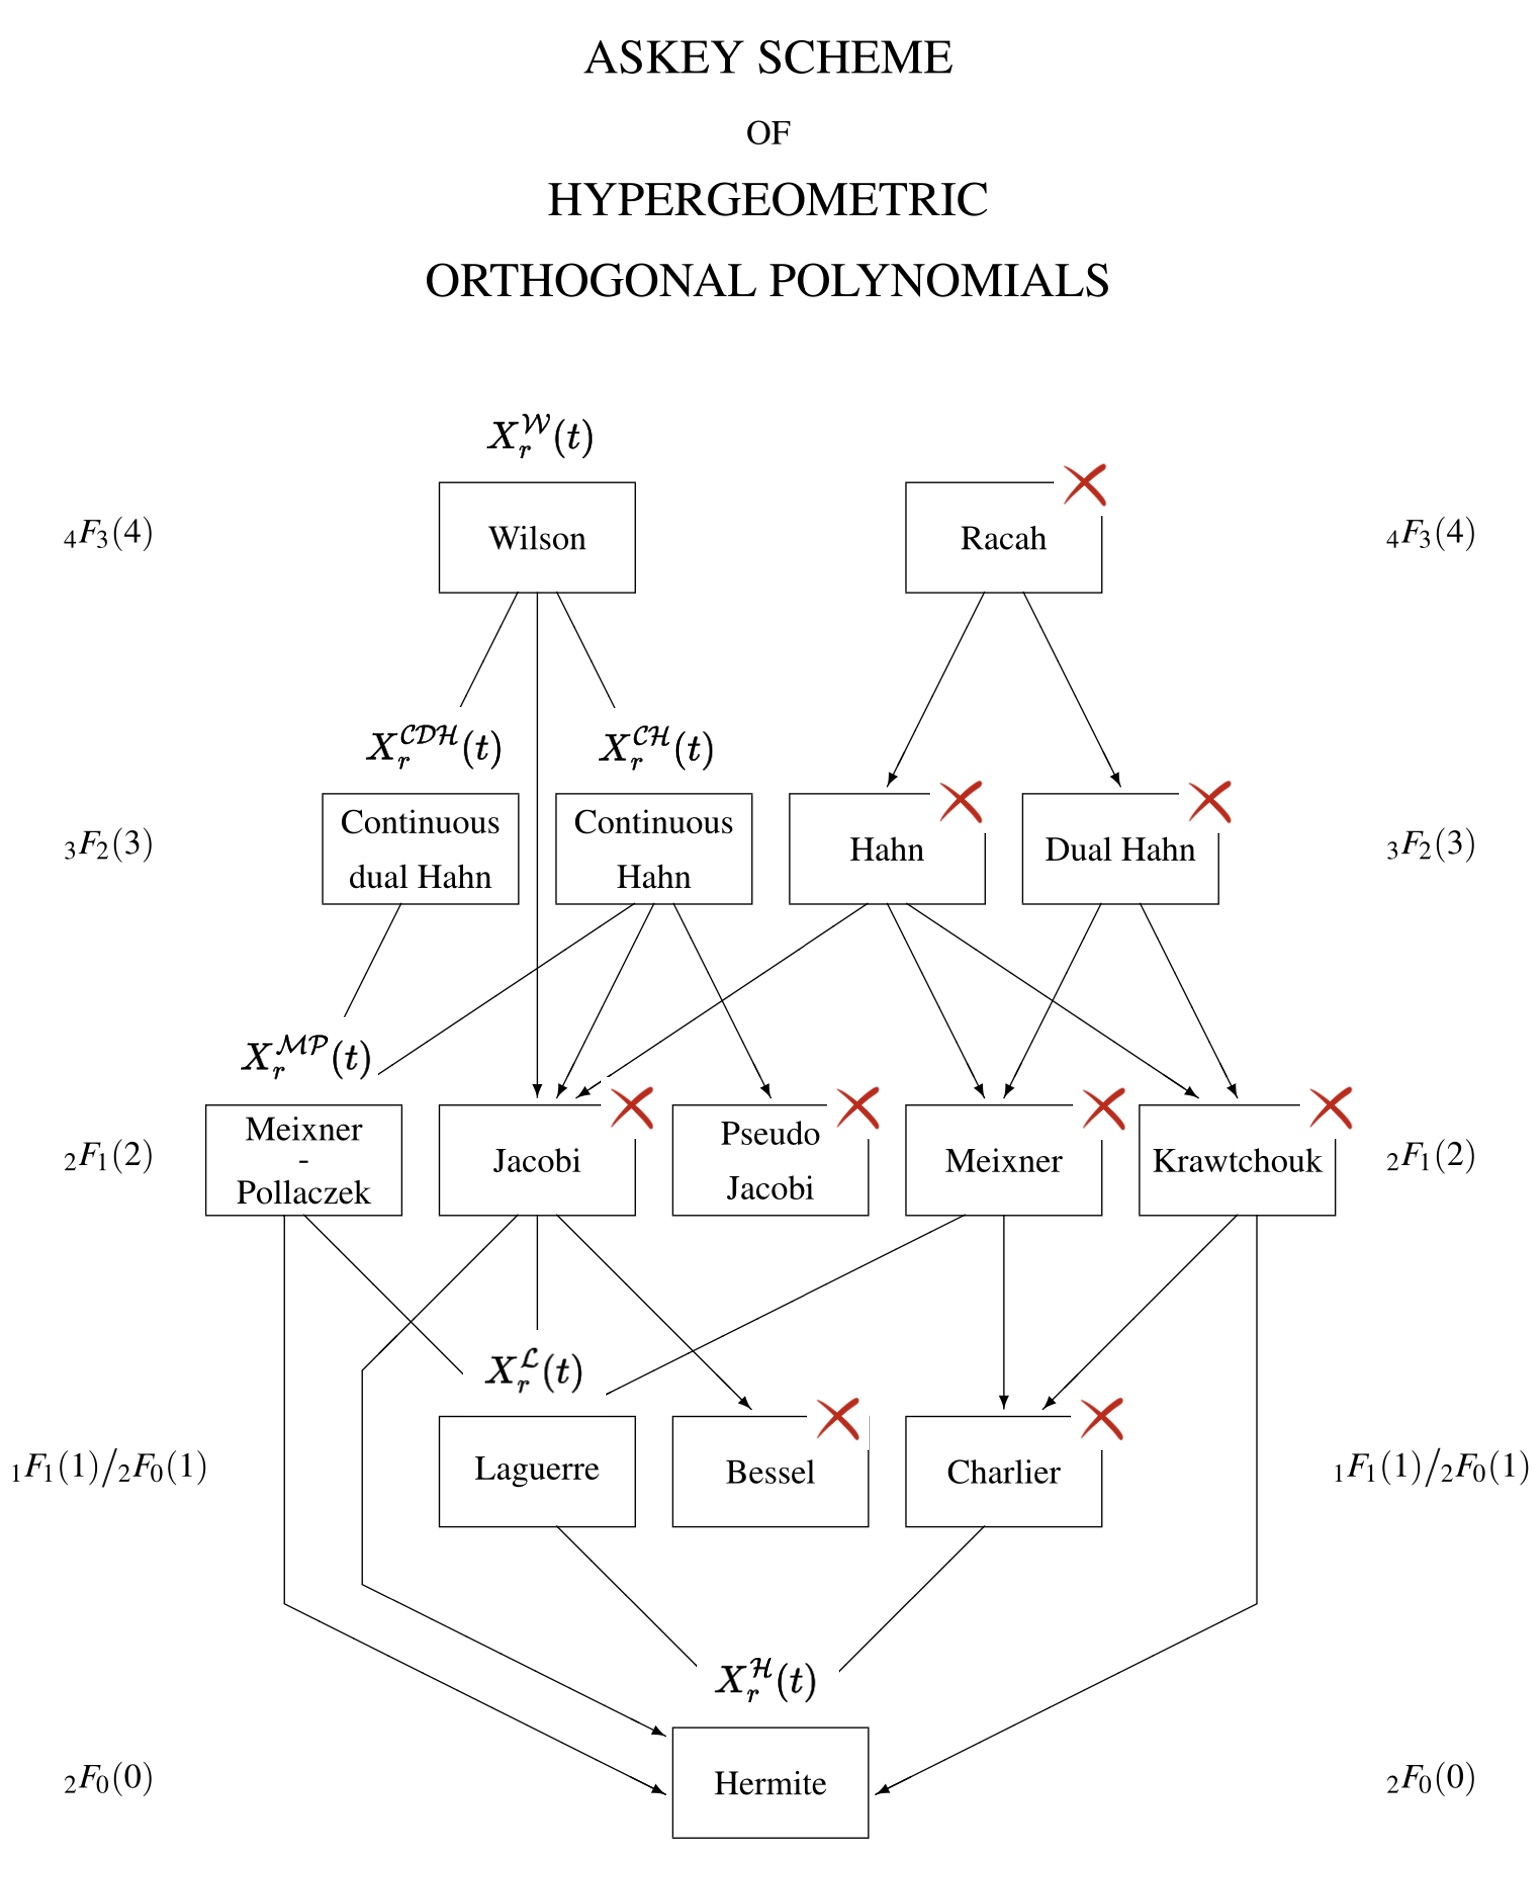
\includegraphics[width=1\linewidth]{Askeyschemenew.jpeg}
  \caption{Askey scheme of orthogonal polynomials. The complexity of the polynomials increases from bottom to top which is reflected in the assocated hypergeometric function. The number between parenthesis reflects the number of free parameters. The arrows always flow from top to bottom and denote possible transformations (mostly based on infinite limits) from one family into another. We have added the labels $X_r^{\mathcal{\Phi}}(t)$ as an easy and unique reference to the Poisson flow connected to a polynomial family. The discrete families have been 'crossed out' from our scope.}
  \label{fig:askey}
\end{figure}

\pagebreak
\section{The Poisson flow} \label{poissonflow}
In paragraph 2.5 of \cite{rom}, Romik introduces the interesting concept of a "Poisson flow". This is based on the idea that any series expansion of the Riemann $\Xi$-function in a system of orthogonal polynomials comes equipped with its own flow based on the standard construction of the so-called Poisson kernel from the theory of orthogonal polynomials. 

We start by denoting $\phi \verifiedeq \left(\phi_n\right)_{n=0}^\infty$ as the family of polynomials that are orthogonal with respect the weight function $w(x)$. The Poisson flow for function $F$ is now defined as follows:
\begin{equation}\label{poiflow}
X^\phi_z(t)\defeq
    \begin{cases}
        \int_{-\infty}^{\infty} p_z(t, \tau)\,F(\tau)\,w(\tau)\,\mathrm{d}\tau & \text{if } 0 < z < 1\\
        \\
        F(t) & \text{if } z = 1
    \end{cases}
\end{equation}

where $F(t)$ is the function to be expanded and $p_z(t, \tau)$ is the Poisson Kernel defined as:
\begin{equation}\label{poiker}
 p^\phi_z(x,y) \defeq \sum_{n=0}^\infty\frac{z^n}{M_n}\, \phi_n(x)\,\phi_n(y)
\end{equation}
with $M_n \verifiedeq \int_\mathbb{R}\phi_n(x)^2\,w(x)\,\mathrm{d}x$. The quantity $M_n$ is the closed form of the orthogonality relation for a polynomial where the two indices are equal. Note that depending on the polynomial family, the integral could also be an infinite sum.

\textit{Remark:} For some families of orthogonal polynomials, the Poisson Kernel $p_z(t, \tau)$ can be expressed into a hypergeometric form. In the literature these are referred to as expressions for "bilinear sums" or "bilinear generating functions" (see for instance \cite{genoverview} and \cite{meipolgen}). We derived a few of these simplified expressions, however they did not provide any benefit for our computations.

Swapping the summation and integration in the Poisson flow (assuming Fubini's theorem applies for $F(t)$), recovers the underlying Fourier series expansion into a family of orthogonal polynomials $\phi$:
\begin{align}
 X^\phi_z(t) &\verifiedeq \sum_{n=0}^\infty z^n\,\gamma_n\,\phi_n(t) \\
 \gamma_n &\verifiedeq \frac{1}{M_n}\,\int_{-\infty}^\infty \Xi(x)\,\phi_n(x)\,w(x) \,\mathrm{d}x
\end{align}

It is this generic structure that we decided to use for our computations, since it allows for the once-off calculation of the coefficients $\gamma_n$ for a certain set of chosen parameters for the orthogonal polynomial under study. All nine orthogonal polynomials in scope can now be expressed into a hypergeometric function and a leading factor $g_n$ that is only dependent on $n$ and the free parameters. This allows us to optimise the coefficient pre-computations a bit further:
\begin{align}
 X^\phi_z(t) &\verifiedeq \sum_{n=0}^\infty z^n\,\gamma_n\,g_n\,{}_pF_q(n,t,\text{parms})\\
 \gamma_n &\verifiedeq  \frac{1}{M_n}\,\int_{-\infty}^\infty \Xi(x)\, g_n\,{}_pF_q(n,x, \text{parms})\,w_n(x) \,\mathrm{d}x
\end{align} 
Collecting all terms that are independent of $r$ and $t$, we will pre-compute $\gamma_n$ as follows:
\begin{align}
 X^\phi_z(t) &\verifiedeq \sum_{n=0}^\infty z^n\,\gamma_n\,{}_pF_q(n,t, \text{parms}) \\
 \gamma_n &\verifiedeq  f_n\,\int_{-\infty}^\infty \Xi(x)\,{}_pF_q(n,x,\text{parms})\,w_n(x) \,\mathrm{d}x \qquad \text{with } f_n = \dfrac{g_n^2}{M_n} 
\end{align} 
\pagebreak

\section{The laws that govern the evolution of the zeros under the Poisson Flow} \label{lawspoissonflow}
When varying parameter $z$ in the Poisson kernel (\ref{poiflow}) between $1$ and $0$, the (real and or complex) zeros of function $F$ at time $z=1$ will start to move. Subsequent changes in $z$ will therefore induce a 'trajectory' of zeros. Trajectories of real zeros can 'collide' (not cross) neighbouring trajectories and transform  into a conjugated pair of complex zeros. An interesting property is 'hyperbolicity, that forces trajectories of zeros, once real, to stay real 'forever'(this can occur moving forwards or backwards in "time" $z$). In this section we aim to derive the laws that govern the flow of zeros expressed into the first derivative of time of a zero at a certain point in time. 

Each family of polynomials in the Askey scheme comes equipped with either a Partial Differential Equation (PDE) or a Differential Difference Equation (DDE). The PDEs can be used to derive the derivative of a specific zero in the flow by expressing it as an infinite \textit{sum} over all zeros to its left and its right ((see chapter 3 of Polymath15 \cite{pol}). The same can be done for the DDEs, but now using an infinite \textit{product} over those zeros (see chapter 3.5 of Romik \cite{rom}). 

A critical first step for deriving the evolution law, is to apply the mapping $$z \rightarrow \exp\left(-r\,(\text{coeff-y})\right) \quad r \in \mathbb{R}. r > 0$$ where \textit{coeff-y} is the coefficient divided by $n$ of $y(x)$ in the DDE or PDE. For some polynomial families this is just $1$, however for others this can become as complex as $\exp\big(n\,(n+\text{parms})\big)$. This should be fine as long as the mapped factor continues to vary sufficiently smooth between $0$ and $1$. We have actually started using the linear variable $z$, however found that using the mapped variable $r$ clearly induces much more 'natural' flows (i.e. resembling the collision patterns of the Pólya-De Bruijn flows) for some of the more complex polynomial families. It therefore seems that this mapped distortion factor provides a more 'natural' way to describe the flow and it also directly paves the way for deriving the governing laws. A rigorous proof for this phenomenon would obviously be desired.    

We will now demonstrate how this works for the Bessel-$y$ (PDE) and the Wilson (DDE) orthogonal polynomial families. The derivation of all the other families follows exactly the same lines and the results have been captured in appendix \ref{eqsused}.

\subsection{Evolution of the zeros under the Bessel $y_n$ Poisson Flow governed by a PDE} \label{Bessellawspoissonflow}
We start from the Bessel $y$ Poisson Flow (\ref{besflow}).
\begin{align}
  M(r,t)=X^{\mathcal{B}}_{r}(t,a) &\verifiedeq \sum_{n=0}^\infty \gamma_n(a)\,{}_2F_0\left([-n, n+a+1],[],-\frac{t}{2}\right)\,\exp(-r(n+a+1))^{n} \quad r \ge 0
\end{align} 

For brevity, we also set $H(t) \defeq {}_2F_0\left([-n, n+a+1],[],-\frac{t}{2}\right)$. 

\begin{lemma}\label{proofBes1} The function $M(r,t)$ satisfies the partial differential equation: 
\begin{align}
 \frac{\partial}{\partial r}M(r,t) \verifiedeq -t^2\,\frac{\partial^2}{\partial t^2}M(r,t) - \big((a+2)\,t+2\big)\,\frac{\partial }{\partial t}M(r,t)
\end{align}
\end{lemma}

\begin{proof}
Using (\ref{besPDE}) we obtain:
\begin{align}
 \frac{\partial}{\partial r}M(r,t) &\verifiedeq  \frac{\partial}{\partial r}\,\left(\sum_{n=0}^\infty \gamma_n(a)\,H(t)\,\exp(-r(n+a+1))^{n}\right) \\
 &\verifiedeq \sum_{n=0}^\infty \gamma_n(a)\,H(t)\,\left(-n\,(n+a+1)\right)\,\exp(-r(n+a+1))^{n} \\
 &\verifiedeq \sum_{n=0}^\infty \gamma_n(a)\,\left(-t^2\,\frac{\partial^2}{\partial t^2}H(t)- \big((a+2)\,t+2\big)\, \frac{\partial}{\partial t}H(t)  \right)\, \exp(-r(n+a+1))^{n}\\
 &\verifiedeq-t^2\,\frac{\partial^2}{\partial t^2}M(r,t) - \big((a+2)\,t+2\big)\,\frac{\partial }{\partial t}M(r,t)
\end{align}
\end{proof}

Now let $z_k(r)$ be the $k$-th simple zero of the flow $M(r,t)$ for a some fixed parameter $a$.
 
\begin{lemma}\label{proofBes2} The evolution of the zeros under the flow $M(r,t)$ is governed by the following equation:
\begin{align}
 \frac{\mathrm{d}}{\mathrm{d} r}z_k(r) \verifiedeq2\, z_k(r)^2\,\sum_{j \ne k}^{'} \frac{1}{z_k(r)-z_j(r)} +(a+2)\,z_k(r)+2
\end{align}
\end{lemma}
where $j \in \mathbb{Z}\backslash\{0\}, j \ne k$. The prime indicates $j$ and $-j$ terms should be summed together (the remaining $k=-j$ term is summed separately).
\begin{proof}
We start from the observation that:
\begin{align}
M(r,z_k(r)) &\verifiedeq 0 \\
\frac{\mathrm{d}}{\mathrm{d} r} \big(M(r,z_k(r))\big) &\verifiedeq 0 \\
\frac{\partial M}{\partial r}(r,z_k(r))+ \frac{\partial M}{\partial t}(r,z_k(r))\,\frac{\mathrm{d} z_k(r)}{\mathrm{d} r} &\verifiedeq 0 \\
t^2\,\frac{\partial^2}{\partial z_k(r)^2}M(r,z_k(r) + \big((a+2)\,z_k(r)+2\big)\,\frac{\partial }{\partial t}M(r,z_k(r))  &\verifiedeq \frac{\partial}{\partial t}M(r,z_k(r))\,\frac{\mathrm{d}}{\mathrm{d} r}z_k(r)
\end{align}

Since we assumed $z_k(r)$ to be simple, its derivative with respect to $t$ can't be zero, hence we can rewrite this as follows:

\begin{align}
\frac{\mathrm{d} }{\mathrm{d} r}z_k(r) &\verifiedeq \dfrac{t^2\,\frac{\partial^2}{\partial t^2}M(r,z_k(r)) + \big((a+2)\,t+2\big)\,\frac{\partial }{\partial t}M(r,z_k(r))}{ \frac{\partial}{\partial t}M(r,z_k(r))} \\
&\verifiedeq z_k(r)^2\,\dfrac{\frac{\partial^2}{\partial t^2}M(r,z_k(r))}{ \frac{\partial}{\partial t}M(r,z_k(r))}  + (a+2)\,z_k(r)+2 \label{secondder}
\end{align}

From Taylor expansion of $M(r,z_k(r)), \frac{\partial}{\partial t}M(r,z_k(r))$ and $\frac{\partial^2}{\partial t^2}M(r,z_k(r))$ around the simple zero $z_k$ we get:
\begin{align}\label{taylor}
 \dfrac{\frac{\partial^2}{\partial t^2}M(r,z_k(r))}{\frac{\partial}{\partial t}M(r,z_k(r))} \verifiedeq 2\,\lim_{z\to z_k} \left(\dfrac{\frac{\partial}{\partial t}M(r,z)}{M(r,z)} -\frac{1}{z - z_k(r)} \right)
\end{align}

We also have the Hadamard product: 
\begin{align}
  M(r,z) \verifiedeq M(r,0)\prod_j^{'}\left(1-\frac{z}{z_j}\right)
\end{align}
where the prime indicates that the $j$ and $-j$ factors are multiplied together. We now take its logarithmic derivative:
\begin{align}
  \dfrac{\frac{\partial}{\partial t}M(r,z)}{M(r,z)} \verifiedeq \sum_j^{'} \frac{1}{z-z_j}
\end{align}
Plugging this into (\ref{taylor}) and then into (\ref{secondder}) gives the result.
\end{proof}

\subsection{Evolution of the zeros under the Wilson Poisson Flow governed by a DDE} \label{Wilsonlawspoissonflow}
We start from the Wilson Poisson Flow (\ref{wilflow}): 
\begin{align}
  M(r,t) \verifiedeq X^\mathcal{W}_{r}(t,a,b,c,d) &= \sum_{n=0}^\infty \gamma_n(a,b,c,d)\,H(t)\,\exp(-r(n+a+b+c+d-1))^{n}
\end{align} 

For brevity we also set $H(t) \defeq {}_4F_3\left(\left[-n, n+a+b+c+d-1,a+it, a- it\right], \left[a+b, a+c, a+d\right], 1\right)$.

\begin{lemma}\label{proofWil1} The function $M(r,t) \verifiedeq X^\mathcal{W}_{r}(t,a,b,c,d)$ satisfies the differential difference equation: 
\begin{align}
 \frac{\partial}{\partial r}M(r,t) \verifiedeq -B(t)\,M(r,t+i) +\left(B(t)+D(t)\right)M(r,t)- D(t)\,M(r,t-i) 
\end{align}
 with $B(t) \verifiedeq \dfrac{(a-it)\,(b-it)\,(c-it)\,(d-it)}{2it(2it-1)}$ and $D(t)=\dfrac{(a+it)\,(b+it)\,(c+it)\,(d+it)}{2it(2it+1)}$.
\end{lemma}

\begin{proof}
Using (\ref{wildde}) we obtain:
\begin{align}
 \frac{\partial}{\partial r}M(r,t) &\verifiedeq  \frac{\partial}{\partial r}\,\left(\sum_{n=0}^\infty \gamma_n(a)\,H(t)\,\exp(-r)^{n\,(n+a+b+c+d-11)}\right) \\
 &\verifiedeq \sum_{n=0}^\infty \gamma_n\,H(t)\,\left(-n\,(n+a+b+c+d-1)\right)\,\exp(-r)^{n\,(n+a+b+c+d-1)} \\
 &\verifiedeq \sum_{n=0}^\infty \gamma_n\,\bigg(-B(t)\,H(t+i) +\left(B(t)+D(t)\right)H(t)- D(t)\,H(t-i)\bigg)\,\exp(-r)^{n\,(n+a+b+c+d-1)}  \\
 &\verifiedeq-B(t)\,M(r,t+i) +\left(B(t)+D(t)\right)M(r,t)- D(t)\,M(r,t-i)
\end{align}
\end{proof}

Now let $z_k(r)$ be the $k$-th simple zero of the flow $M(r,t)$ for a some fixed set of parameters $a,b,c,d$.
 
\begin{lemma}\label{proofWil2} The evolution of the zeros under the Wilson Poisson flow $M(r,t)$ is governed by the following equation:
\begin{align}
 \frac{\mathrm{d}}{\mathrm{d} r}z_k(r) \verifiedeq i\,B(z_k(r))\, \prod^{'}_{j \ne k}\left(1+ \frac{i}{z_k(r)-z_j(r)}\right) -i\,D(z_k(r))\,\prod^{'}_{j \ne k} \left(1-\frac{i}{z_k(r)-z_j(r)}\right)
\end{align}
\end{lemma}
where $j \in \mathbb{Z}\backslash\{0\}, j \ne k$. The prime indicates $j$ and $-j$ terms should be multiplied together (the remaining $k=-j$ term is multiplied separately).
\begin{proof}
We start from the observation that:
\begin{align}
M(r,z_k(r)) &\verifiedeq 0 \\
\frac{\mathrm{d}}{\mathrm{d} r} \big(M(r,z_k(r))\big) &\verifiedeq 0 \\
\frac{\partial M}{\partial r}(r,Z_k(r))+ \frac{\partial M}{\partial t}(r,z_k(r))\,\frac{\mathrm{d} z_k(r)}{\mathrm{d} r} &\verifiedeq 0 \\
B(z_k(r))\,M(r,z_k(r)+i) + D(z_k(r))\,M(r,z_k(r)-i)  &\verifiedeq \frac{\partial}{\partial t}M(r,z_k(r))\,\frac{\mathrm{d}}{\mathrm{d} r}z_k(r)
\end{align}

Since we assumed $z_k(r)$ to be simple, its derivative with respect to $t$ can't be zero, hence we can rewrite this as follows into the DDE:

\begin{align} \label{WilDDE1}
\frac{\mathrm{d} }{\mathrm{d} r}z_k(r) &\verifiedeq \dfrac{B(z_k(r))\,M(r,z_k(r)+i) + D(z_k(r))\,M(r,z_k(r)-i)}{ \frac{\partial}{\partial t}M(r,z_k(r))}
\end{align}

For the next step we follow the same approach as Romik [ref]. We consider the finite entire function:

\begin{align}
M_p(r,t) \verifiedeq \sum_{k=0}^n \gamma_n \, H(t)\,\exp(-r(n+a+b+c+d-1))^{n} 
\end{align}

defined as a solution to the DDE (\ref{WilDDE1}), where $p(t) \defeq \prod_{k=1}^n(t-z_k)$ and the initial condition $M_p(0,t) \defeq p(t)$. 

We have the factorisation and its derivative: 
\begin{align}
M_p(r,t) &\verifiedeq \exp(-r)^{n\,(n+a+b+c+d-1)}\,\prod_{j=1}^n\bigg(t-z_j(r)\bigg)\\
\frac{\partial}{\partial t} M_p(r,z_k(r)) &\verifiedeq \exp\left(-r(n+a+b+c+d-1)\right)^{n}\,\prod^n_{\substack{j=1\\j\ne k}}\bigg(z_k(r)-z_j(r)\bigg)
\end{align}

Taking $n \rightarrow \infty$ and plugging this into (\ref{WilDDE1}) gives the result:

\begin{align} \label{WilDDE2}
 \frac{\mathrm{d}}{\mathrm{d} r}z_k(r) \verifiedeq i\,B(z_k(r))\, \prod^{'}_{j \ne k} \frac{z_k(r)+i-z_j(r)}{z_k(r)-z_j(r)} -i\,D(z_k(r))\,\prod^{'}_{j \ne k} \frac{z_k(r)-i-z_j(r)}{z_k(r)-z_j(r)}
\end{align}
\end{proof}

\section{The functions to be expanded: Riemann $\Xi(t)$ and $\Xi_i(t)$} \label{functobexpanded}
Our main focus will be on expanding the Riemann $\Xi(t)$ function and to visualise its flows. Since our framework is generic, we decided to include a similar, yet much simpler function in our scope and to compare the results. We know that the non-trivial zeros $\rho_n$ of $\xi(s)$ determine the oscillation (error) term in the prime counting function(s). Analogously, the equidistant zeros $\mu_n\verifiedeq 0 \pm 2\pi n i$ induce the oscillating term (sawtooth shaped) in the integer counting function. The entire function associated with the Hadamard product of these $\mu$'s is $\xi_i(s) \defeq \frac{2}{s}\sinh\left(\frac{s}{2}\right)$. Analogously to $\Xi(t)$, we can define $\Xi_i(t) \defeq  \xi_i\left(it\right) \defeq \frac{t}{2}\sin\left(\frac{t}{2}\right)$. The main properties of both functions are summarised in table \ref{tab:tablefunc}.

\small{
\begin{table}[H]
  \begin{center}
    \caption{Properties of the selected functions and the Pólya-De Bruijn flow}
    \label{tab:tablefunc}
    \begin{tabular}{|c|c|} 
      $F\verifiedeq\Xi(t)$ & $F\verifiedeq\Xi_i(t)$\\
      \hline
       & \\
      $ \xi(s) \defeq \displaystyle \frac{s\,(s-1)}{2} \,\pi^{-s/2}\, \Gamma\left(\frac{s}{2}\right)\, \zeta(s)$ & $\xi_i(s) \defeq\displaystyle \frac{2}{s}\,\sinh\left(\frac{s}{2}\right)$ \\ 
       & \\
      $ \displaystyle \Xi(t)\defeq\xi\left(\frac12+it\right)$ & $\displaystyle \Xi_i(t)\defeq \xi_i\left(it\right)\defeq\frac{2}{t}\,\sin\left(\frac{t}{2}\right)$ \\
       & \\
      $ \displaystyle \Xi(t) \verifiedeq \Xi(-t)$ & $\displaystyle \Xi_i(t) \verifiedeq \Xi_i(-t)$ \\
       & \\
      $ \displaystyle \Xi(\overline{t}) \verifiedeq \overline{\Xi(t)}$ & $\displaystyle \Xi_i(\overline{t}) \verifiedeq \overline{\Xi_i(t)}$ \\
       & \\
      $ \displaystyle \Xi(t) \verifiedeq \Xi(0)\,\prod_n \left(1-\dfrac{t}{\Im(\rho_n)}\right)\left(1+\dfrac{t}{\Im(\rho_n)}\right)$ & $\displaystyle \Xi_i(t) \verifiedeq \Xi_i(0)\,\prod_n \left(1-\dfrac{t}{\mu_n}\right)\left(1+\dfrac{t}{\mu_n}\right)$\\
       & \\
      $ \Xi(t) \verifiedeq\displaystyle 2\int_0^\infty \Phi(x)\, \cos(t\,x)\, dx$ & $\Xi_i(t) \verifiedeq\displaystyle 2\,\int_0^{\frac12} \Phi_i(x)\, \cos\left(t\,x\right)\, dx$ \\
       & \\
      $\Phi(x)\verifiedeq\displaystyle 2\sum_{n=1}^\infty \left(2\,\pi^2\,  n^4\, \mathrm{e}^{9x/2} - 3\,\pi\, n^2\, \mathrm{e}^{5x/2} \right) \mathrm{e}^{-\pi\, n^2 \mathrm{e}^{2x}}$  & $\displaystyle \Phi_i(x)\verifiedeq1$ \\
       & \\
      $\displaystyle \Xi_{\lambda}(t) \verifiedeq \frac{1}{\sqrt{\pi}}\int_{-\infty}^\infty \Xi\left(t - 2\,i\,x\sqrt{\lambda}\right)\mathrm{e}^{-x^2}\mathrm{d}x$ & $\displaystyle \Xi_{i\,\lambda}(t) \verifiedeq \frac{1}{\sqrt{\pi}}\int_{-\infty}^\infty \Xi_i\left(t - 2\,i\,x\sqrt{\lambda}\right)\mathrm{e}^{-x^2}\mathrm{d}x$ \\
       & \\
      $\displaystyle \frac{\partial^1}{\partial \lambda^1} \Xi_{\lambda}(t) \verifiedeq -\,\frac{\partial^{2}}{\partial t^{2}} \Xi_{\lambda}(t)$  & $\displaystyle \frac{\partial^1}{\partial \lambda^1} \Xi_{i\,\lambda}(t) \verifiedeq -\,\frac{\partial^{2}}{\partial t^{2}} \Xi_{i\,\lambda}(t)$\\
       & \\
       \hline
    \end{tabular}
  \end{center}
\end{table}
}
\pagebreak

In figure \ref{fig:poldebruijnflow} we visualise the Pólya-De Bruijn flows for $\Xi_{\lambda}(t)$ and $\Xi_{i\,\lambda}(t)$. Vestiges of the distinct pattern of the first graph, will re-emerge in the visualisation of the flows of other polynomial expansions.

\begin{figure}[H]
  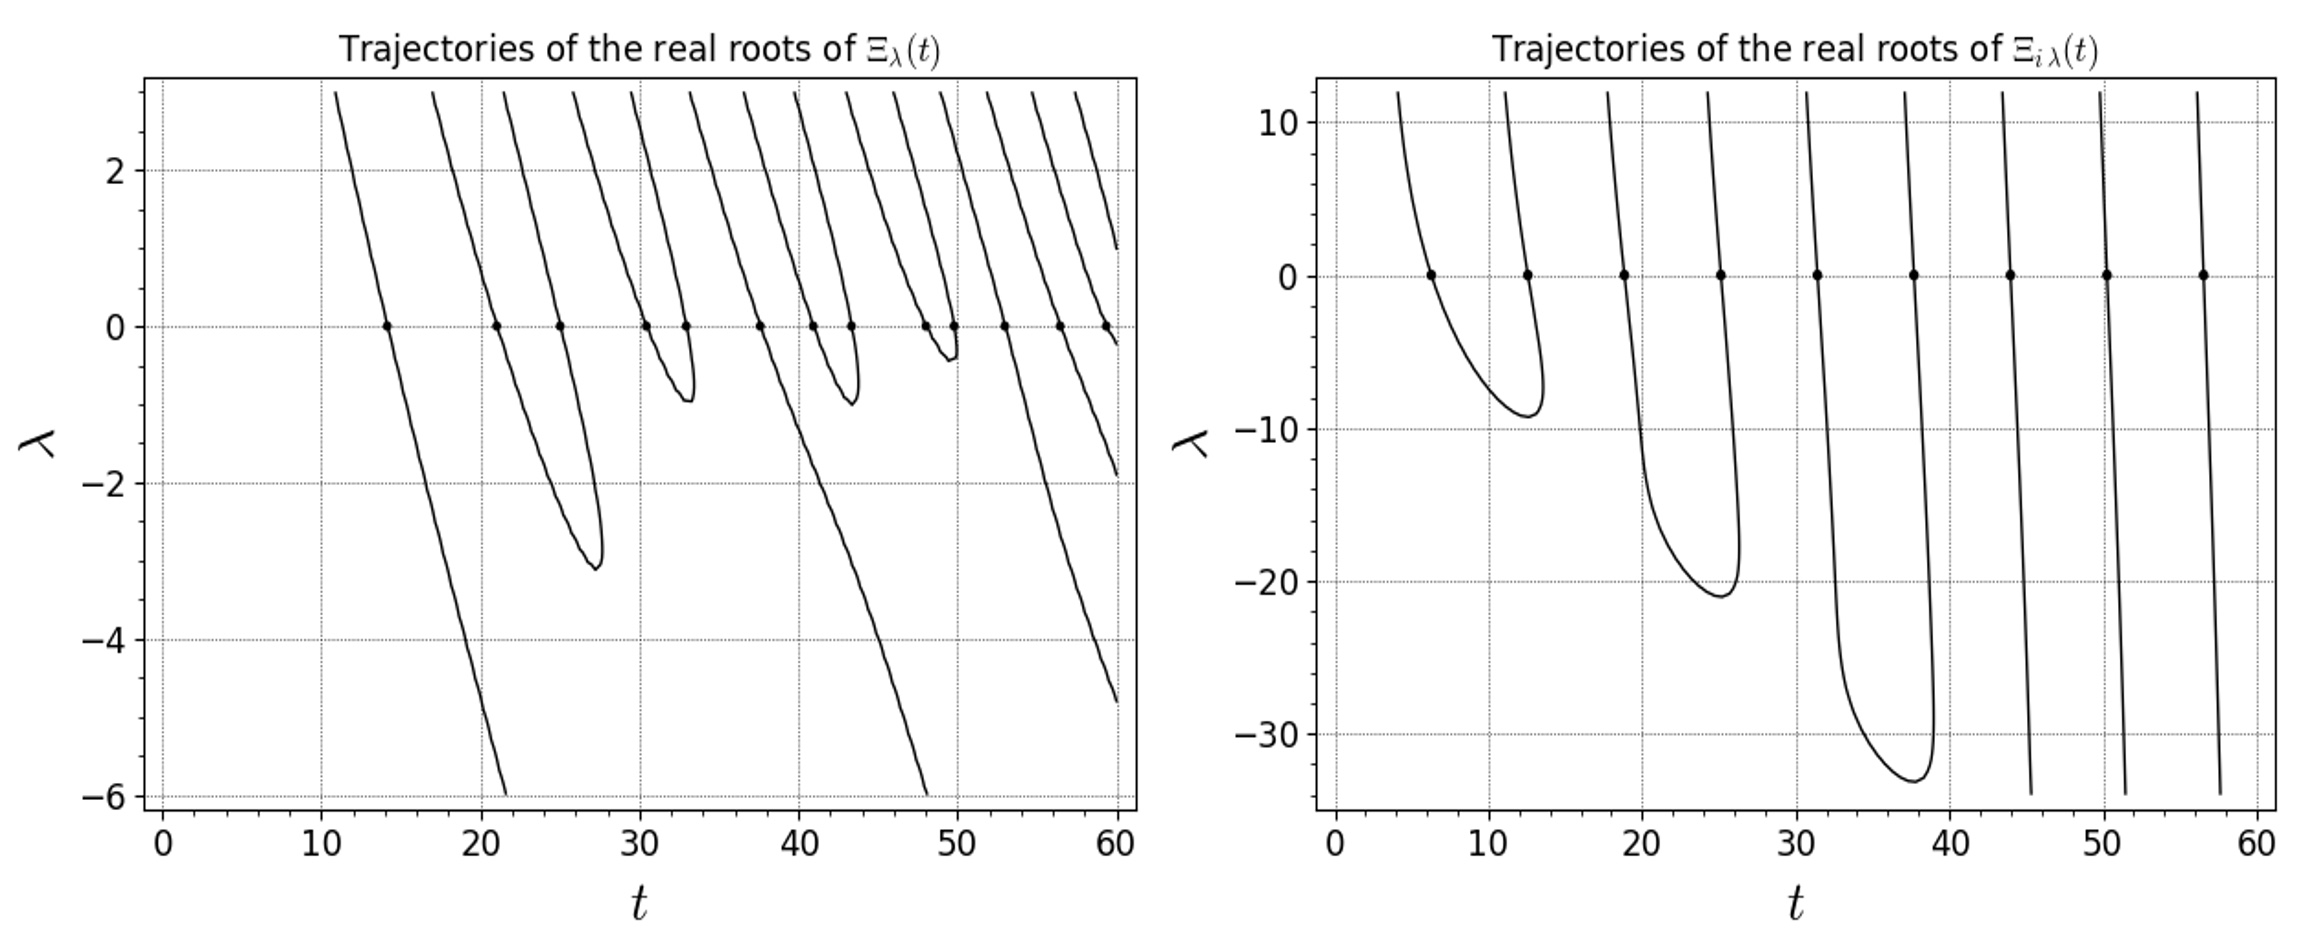
\includegraphics[width=1\linewidth]{PolyaDeBruijnFlowdouble.jpeg}
  \caption{The graphs show the DeBruijn-Newman flows of real zeros of $\Xi_{\lambda}(t)$ (left) and $\Xi_{i\,\lambda}(t)$ (right). Some collisions occur between the trajectories when $\lambda < 0$ and we were surprised to see those also in right graph, even though the initial zeros are regularly spaced. The collision point is where the real zeros transform into a complex pair when going further back in 'time'. The RH is equivalent to no collisions occurring for $\lambda \ge 0$, which is clearly true for $\Xi_{i\,\lambda}(t)$. The concept of "hyperbolicity", i.e. the preservation of the reality of the zeros when time-parameter $\lambda$ become more positives, is clearly visible in both flows.}
  \label{fig:poldebruijnflow}
\end{figure}

A few facts about the flow of $\Xi_{\lambda}(t)$:
\begin{itemize}
  \item De Bruijn and Newman showed that there exists a constant $\Lambda$, now known as the De Bruijn-Newman constant, at which all zeros will be real and that this is also true for all $\lambda > \Lambda$. During the last decades, good progress has been made on the improvement of the lower bound of $\Lambda$, however only a minor reduction was scraped off the upper bound ($<0.5$ instead of $\le 0.5$).
  \item In 2018 Tao and Rodgers \cite{rot} proved Newman's lower bound conjecture that $\Lambda \ge 0$, They used techniques from Random Matrix theory to predict the 'time to cool down' and compared this to known facts about the distribution of zeros at $\lambda = 0$. A student of Tao, Alex Dobner later found a much simpler proof \cite{dob} that $\Lambda \ge 0$ which avoids the heat equation approach. Dobner’s approach instead relies on a Riemann-Siegel type approximation for $\Xi_{\Lambda}(t)$ in order to demonstrate the existence of zeros off the critical line.
   \item The prime objective of the 2018 Polymath15 project \cite{pol}, was to lower the upper bound. This was successfully accomplished through a combination of analytic proof, existing numerical verification of the RH up to a certain height and advanced computer calculations. The new upper bound became $\Lambda \verifiedeq 0.22$. After further numerical verification of the RH by Platt et al \cite{pla}, it has now been proven that the upper bound of the De Bruijn-Newman constant is $\lambda \le 0.2$. Hence, a breach of the RH would imply that there exists some pair complex zeros at a certain $T$ that collide in the region $0 \le \Xi_{\lambda}(t) \le 0.2$.
  \item For increasingly positive $\lambda$ we know that the trajectories of zeros "cool down" into a deterministic arithmetic progression that is now well understood.
  \item Increasingly negative $\lambda$ will induce more pairs of complex zeros that eventually will organise themselves on deterministic curves. A sparse, but regular set of real zeros (see the $1$-st and $6$-th trajectories in the graph) remains real 'forever' (probably because they are initially already too far apart to be able to collide). 
\end{itemize}

\pagebreak

\section{Mathematical considerations}\label{mathcons}
The functions $\Xi(t)$ and $\Xi_i(t)$ need to comply with the following:
\begin{enumerate}
\item Its expansion has to be convergent everywhere in $\mathbb{C}$.
\item Fubini's theorem should hold when swapping summation and integration.
\item All zeros in the flow must be simple to ensure their first derivative is $\ne 0$.
\item For Hadamard factorisation, the flow must be even, non-zero at the origin and entire of order $1$. 
\end{enumerate} 

The disadvantage of our generic approach is that the Riemann $\Xi(t)$ function appears in the coefficients. This makes the task of providing a rigorous proof for 1) and 2) much more difficult. Romik showed in his paper how to derive much simpler expressions for the coefficients that enable a rigorous proof of 1) and 2) and also pave the way for deriving their asymptotics. Following the same techniques, we managed to generalise his approach towards a broader set of parameters for Meixner-Pollaczek and Continuous Hahn families. We also found similar expressions for the coefficients of the Generalised Laguerre, Continuous Dual Hahn and Wilson polynomials, albeit for the latter two for $\Xi'(t)/t$ and $\Xi(0) \pm \Xi(t)$ and with a restricted set of parameters. We've captured these in appendix \ref{specexpansions}. Since this approach does not provide access to all continuous orthogonal polynomial flows that we aim to visualise and our domain of interest is $t < 60$, we decided to just assume that 1) and 2) to be true at this stage.

For $\Xi(t)$ it is still an open problem whether all its zeros are simple, however in our domain of interest $t < 60$ this is true. Also, it is known that 4) holds for $\Xi(t)$ and $\Xi_i(t)$.    

\section{Computational considerations}\label{compcons}
Visualising the Poisson flow of the Riemann $\Xi$ and $\Xi_i$-functions requires a significant amount of evaluations of the function itself as well as the hypergeometric functions associated with the family of orthogonal polynomials. During the Polymath15 project we discovered that with modern software and hardware evaluating $\Xi$ actually has become quite tractable at smaller heights (p16, remark 4.1 of \cite{pol}). 

The most intense task is to pre-compute and store the coefficients (for each set of polynomial parameters) that are independent of $t, r$. This once-off computation makes the evaluation of the flow $X^\phi_r(t)$ significantly faster since only one hypergeometric function remains. For both steps we have used the advanced FLINT/ARB C-library for arbitrary-precision ball arithmetic \cite{arb}. We have also considered using pari/gp and, although much easier to code, it proved to be slower and lacks some of the more advanced hypergeometric functions (${}_3F_2,{}_4F_3$) that we need.

For the pre-computation step we require the full FLINT/ARB C-library and especially the multi-threaded function for the fast evaluation of the integral. This multi-threaded function seems not (yet) available in the 'wrapped', easier readable, version of FLINT/ARB under SageMath, hence we coded it all in "plain ARB". For the flow visualisation step, we make use of Sagemath \textit{implicit plot} function that automatically plots where the contour of a function vanishes. There is no longer a need for dedicated root finding routines and this again speeds up computations considerably. To allow for easy integration between evaluating and plotting the Poisson flow, we made use of the "wrapped" version of FLINT/ARB under SageMath.    

To keep a decent balance between gaining sufficient visual insights and the amount of computations required, we decided to compute the flows up to $t=60$ which comprises the flows of the first $13$ ordinates of the non-trivial zeros of $\Xi(t)$ at $r=0$. Our target accuracy at $t=60, r=0$ is $20$ digits, which allows for some contingency to 'peek' beyond that point. The key tuning parameters to achieve this accuracy are the number of pre-computed coefficients, the precision settings in the software and the finite limits of the integrals/sums involved. Finding the right settings was done heuristically. 

For the hardware we have used an Apple Mac Studio, M2 ultra, 64Gb, using all its 24 cores to the max. All documented software, including the accuracy settings that we have used to pre-compute the coefficients and to produce the visuals, is available from our GitHub \cite{git} repository. All pre-computed coefficients and other relevant data are stored there as well.

\section{Verifying the results}\label{checks}
We have implemented the following checks to ensure the computations were done correctly:

\begin{enumerate}
\item \textit{Ensure the code produces replicable results.} We verified the correct working our FLINT/ARB code by fully reproducing it in Maple\texttrademark  \cite{map} and comparing randomly chosen values. 
\item  \textit{Verify the expansion meets the target accuracy of $20$ digits.} Check that the difference $F(60)-X^\phi_0(60)$ shows at least $20$ zeros.
\item  \textit{Verify the expansion has been done correctly.} Check that $F(t) \verifiedeq \sum_{n=0}^\infty (\text{coefficient}_n)$ at $t=0$ (Hermite, Bessel and Laguerre), at $t=1$ (Jacobi), at $t=i$ (Pseudo Jacobi) and at $t\verifiedeq ai$ (Meixner-Pollaczek, Continuous Hahn, Continuous Dual Hahn and Wilson polynomials). 
\item \textit{Verify that the derived expressions for $\frac{d}{d\,r}z_k(r)$ work correctly.}. Check that the Newton approximation of the first derivative at a known $k$-th zero of $F$ at $r=0$, equals the value of the derived equation for $\frac{d}{d\,r}z_k(0)$. For brevity let $z_n = z_n(0)$. 

For the PDEs we evaluate the sum of zeros for $F=\Xi(t), z_n=\Im(\rho_n)$ and $F=\Xi_i(t), z_n=2\pi n$ respectively as:
\begin{align}
 \sum_{j \ne k}^{'} \frac{1}{z_k-z_j} &\verifiedeq \left(\sum_{j =1}^{k-1} \left(\frac{1}{z_k-z_j}\right)+\left(\frac{1}{z_k+z_j}\right)\right) +\left(\sum_{j = k+1}^{100000} \left(\frac{1}{z_k-z_j}\right)+\left(\frac{1}{z_k+z_j}\right)\right)+\left(\frac{1}{2\,z_k} \right) \notag \\
  \sum_{j \ne k}^{'} \frac{1}{z_k-z_j} &\verifiedeq -\frac{1}{2\pi k} \notag
\end{align}
For the DDEs we evaluate the product of zeros $F\verifiedeq \Xi(t), z_n=\Im(\rho_n)$ and $F=\Xi_i(t), z_n=2\pi n$ respectively as (note: $c \verifiedeq \pm 1$ or $c =\pm i$):
\begin{align}
 \prod_{j \ne k}^{'} \frac{z_k+c-z_j}{z_k-z_j} &\verifiedeq c\,\left(\prod_{j =1}^{k-1} \left(1+\frac{c}{z_k-z_j}\right)\,\left(1+\frac{c}{z_k+z_j}\right)\right)\,\left(\prod_{j = k+1}^{100000} \left(1+\frac{c}{z_k-z_j}\right)\,\left(1+\frac{c}{z_k+z_j}\right)\right)\,\left(1+\frac{c}{2\,z_k} \right) \notag \\
 \prod_{j \ne k}^{'} \frac{z_k+c-z_j}{z_k-z_j} &\verifiedeq 2\,k\,\pi\,c^4\,(-1)^k\,\frac{\sin\left(\pi\,k+\dfrac{c}{2}\right)}{\pi\,k+\dfrac{c}{2}} \notag
\end{align}
\end{enumerate}

\section{Overview of the results} \label{results}
In appendix \ref{eqsused}, we list all relevant equations for each orthogonal polynomial family in scope. The visuals of the flows are also included there. For the Generalised Laguerre, Bessel, Jacobi and Pseudo-Jacobi families, we found that computing the $\frac{\partial^{d}}{\partial t^{d}} X^{\mathcal{\phi}}_r(t)$, where $d$ is the $d$-th partial $t$-derivative of the flow, could be done almost for "free". For these families we have included (but not coded) these extended equations.  

Formally, the flows should only be valid for $r > 0$, however computations showed that these could be extended into the negative domain yielding further insights. For $F=\Xi(t)$ we see two types of flows in the domain $r > 0$:
\begin{itemize}
  \item \textit{Type A:} All collisions seem to occur here (and no collisions for $r < 0$).
  \item \textit{Type B:} No collisions seem to occur here (and all collisions for $r < 0$).
\end{itemize}

Note that to properly compare the new Poisson flows with the Polya-De Bruijn flow, the latter should be vertically "flipped" ($\lambda = -\lambda$) so it becomes a type A. The reason is the negative mapping $\exp(-r)$ that we have applied to the other Poisson flows. 

In the table \ref{tab:tablefindings} we summarize the flow type we see for each family. We also include an observation about the behaviour of the coefficients (i.e. whether they are always positive/negative/alternating and/or increase/decrease monotone).

\begin{table}[H]
  \begin{center}
    \caption{Overview of our findings ordered by flow type }
    \label{tab:tablefindings}
    \begin{tabular}{l|l|c|l|} 
      Polynomial & Flow & Type & Coefficients\\
      \hline
      Pólya-De Bruijn & $\Xi_{\lambda}(t)$ & A\\
      Hermite & $X^\mathcal{H}_r(t)$  & A & Odd index $= 0$, all positive real, monotone decreasing\\
      Laguerre & $X^\mathcal{L}_r(t)$  & A & Alternating with decreasing frequency, no pattern observed\\
      Bessel-y & $X^\mathcal{B}_r(t)$  & B & Alternating + + - -, monotone decreasing\\
      Meixner Poll. & $X^\mathcal{MP}_r(t)$  & B & Odd index $= 0$, all positive real, monotone decreasing\\
      Pseudo-Jacobi & $X^\mathcal{PJ}_r(t)$  & B & All complex, real part positive, imaginary part alternating + -\\      
      Jacobi & $X^\mathcal{J}_r(t)$  & B & Odd index $= 0$ when $\alpha = \beta$, alternating + -, monotone decreasing\\
      Cont. Dual Hahn & $X^\mathcal{CDH}_r(t)$  & B & All positive real, monotone decreasing\\
      Cont. Hahn & $X^\mathcal{CH}_r(t)$  & B & Odd index $= 0$, all positive real, monotone decreasing\\
      Wilson & $X^\mathcal{W}_r(t)$  & B & All positive real, monotone decreasing\\
    \end{tabular}
  \end{center}
\end{table}


\section{Discussion and concluding remarks}\label{concremarks}

We have demonstrated that visualising the Poisson flows is computationally tractable at limited heights. The visualised flows could provide potentially new perspectives on the evolution of the real zeros of $\Xi(t)$ and $\Xi_i(t)$ as well as their governing laws. In this section we summarise a few of our key insights.
 
\begin{itemize}
  \item We start with a realistic observation. The common characteristic of all Poisson flows is that they start off with a distortion/approximation of the original functions $\Xi(t), \Xi_i(t)$ at $r=0$ where the complexity already seems highest. We observe that over time, information seems to flow from $r=0$ towards later or earlier phases. In these less complex 'distorted' domains ($r \ne 0$) we see trajectories either collide or converge towards an arithmetic progression. Unfortunately, we do not (yet) see any information gained from this 'distorted' domain that could tell us more about the distribution of the zeros at $r=0$. 
\item However, on a more positive note, we find it really encouraging to see that the visualised flows for each expansion can be categorised into two distinct types and this raises new questions. What is the mechanism that induces these two types of flows? What makes for instance the one-parameter Generalised Laguerre and Bessel-$y$ families so different? Their PDEs tell us whether the flows are skewed to the left or to the right, however they don't explain whether collisions should occur in domain $r < 0$ or $r > 0$. 
\item Romik demonstrates in section 3.5 of \cite{rom}, that the Differential Difference Equation (DDE) that underpins the dynamical evolution of the real zeros of the Meixner Pollaczek expansion no longer preserves the property of "hyperbolicity". However, the visualised Poisson flow suggests that a form of "hyperbolicity" is being preserved, but into the positive direction of "time" $r$. We observe the same for the other family's DDEs: in the domain $r > 0$ the flows tend to 'cool down' with time and trajectories of real zeros eventually organise themselves into an arithmetic progression. Could it be that "hyperbolicity" is maintained for $r > 0$ ? 
\item In chapter 7 "Final remarks" of \cite{rom}, Romik makes the observation that:
\begin{quotation}
\textit{One rather striking fact is that the four different series expansions} (i.e. Pólya-De Bruijn, Hermite, Meixner Pollaczek, Continuous Hahn) \textit{we have considered for the Riemann $\Xi$ function, exhibit remarkably similar structural similarities: namely, in all four expansions the coefficients appear with alternating signs (and their asymptotics can be understood to a good level of accuracy, as our analysis shows). It is intriguing to wonder about the significance of this structural property of $\Xi(t)$. Can this information be exploited somehow to derive information about the location of the zeros of $\Xi(t)$? By way of comparison, one can consider “toy” expansions of the above forms involving more elementary coefficient sequences.}
\end{quotation}

\pagebreak
He then shows the (trivial) reality of the zeros for all families, except for the Continuous Hahn polynomials. This raises the question whether anything could be said about the reality of the zeros of the $g_n$ polynomial expansion (i.e. the Continuous Hahn polynomials with parameters $\frac34, \frac34, \frac34, \frac34$). We found that after a slight change of parameters, it becomes quite easy to show that all zeros of the alternating generating function of the Continuous Hahn polynomial are real and regularly spaced for all $0 < r < 1$. We start from equation 9.4.11 in \cite{koe} and have:
\begin{align}
\sum_{n=0}^\infty (-1)^n\, \frac{(2)_{2n}}{\left(\frac32\right)_{2n}}\frac{ r^{2n}}{(2n)!}p_{2n}^{\left(\frac12,1,\frac12,1\right)}(t) &\verifiedeq \frac12\,\left(\frac{{}_2F_1\left(\left[1,\frac12-it\right],\left[1\right], -\frac{4r}{(1-r)^2}\right)}{(1-r)^2}+\frac{{}_2F_1\left(\left[1,\frac12-it\right],\left[1\right], \frac{4r}{(1+r)^2}\right)}{(1+r)^2} \right) \\
 & \verifiedeq \frac12\, \left(\frac{1}{\left(1-r \right)^{2}}\,\left(\left(\dfrac{r+1}{r -1}\right)^{2}\right)^{-\frac{1}{2}+it}+\frac{1}{{\left(1+r \right)^{2}}}\,\left(\left(\dfrac{r -1}{r+1}\right)^{2}\right)^{-\frac{1}{2}+it}\right) \notag
\end{align}

where the last equation has only real zeros (see table \ref{tab:tablezeros}).

We onbserved that also the Jacobi polynomials possess the property that the coefficients at odd indices are zero (but only when $\alpha\verifiedeq \beta$). Using equation 9.8.13 in \cite{koe} yields its toy expression for $\alpha \verifiedeq \beta\verifiedeq \frac12$:

\begin{align}
\sum_{n=0}^\infty (-1)^n \frac{(2)_{2n}}{\left(\frac32\right)_{2n}}r^{2n}\,P_{2n}^{\left(\frac12,\frac12\right)}(t) &\verifiedeq \frac12\,\left(\frac{{}_2F_1\left(\left[1,\frac32\right],\left[\frac32\right],\frac{ir\,2(t-1)}{(1-ir)^2}\right)}{(1-ir)^2}+\frac{{}_2F_1\left(\left[1,\frac32\right],\left[\frac32\right], \frac{-ir\,2(t-1)}{(1+ir)^2}\right)}{(1+ir)^2}\, \right) \\
  & \verifiedeq \frac{\left(1-r^2\right)}{1+r^4+r^2\left(4\,t^2-2\right)} \notag
\end{align}

where the last equation has no zeros.

This results in the extended list of "toy" expansions and the closed forms for their $n-$th zero (all real and simple):
\begin{table}[H]
  \begin{center}
    \caption{"Toy" expansions and the reality of their zeros}
    \label{tab:tablezeros}
    \begin{tabular}{l|l|l|} 
      Polynomial & Toy expansion for $0 < r < 1$ & Formula for  $n$-th zero, $ n \in \mathbb{Z}, r \in \mathbb{R}$\\
      \hline
      "Polya De Bruijn" & $\displaystyle \sum_{n=0}^\infty (-1)^n\, \frac{ r^{2n}}{(2n)!}\,t^{2n}$  &$\displaystyle z_n(r) \verifiedeq \dfrac{\pi  \left(n-\frac12\right)}{r}$ \\       
      Hermite & $\displaystyle \sum_{n=0}^\infty (-1)^n\, \frac{ r^{2n}}{(2n)!}\, H_{2n}\left(t\right)$  &$\displaystyle z_n(r) \verifiedeq \dfrac{\pi  \left(n-\frac12\right)}{2r}$ \\
      Meixner Pollaczek & $\displaystyle \sum_{n=0}^\infty (-1)^n\, r^{2n}\, P_{2n}^{\left(\frac34\right)}\left(t, \frac{\pi}{2}\right)$ &  $\displaystyle z_n(r) \verifiedeq \dfrac{\pi  \left(n-\frac12\right)}{\mathrm{log}\! \left(\dfrac{1+r}{1-r}\right)}$\\
      Continuous Hahn & $\displaystyle \sum_{n=0}^\infty (-1)^n\, \frac{2n+1}{\left(\frac32\right)_{2n}}\,r^{2n}\,p_{2n}\left(t,\frac12,1,\frac12,1\right)$  & $\displaystyle z_n(r) \verifiedeq \dfrac{\pi  \left(n-\frac12\right)}{\mathrm{log}\! \left(\dfrac{r +1}{r-1}\right)-\mathrm{log}\! \left(\dfrac{r-1}{r+1}\right)}$\\
     Jacobi & $\displaystyle \sum_{n=0}^\infty (-1)^n\, \frac{(2)_{2n}}{\left(\frac32\right)_{2n}}\,r^{2n}\,P_{2n}^{\left(\frac12,\frac12\right)}(t)$  & no zeros at all\\
    \end{tabular}
  \end{center}
\end{table}

\pagebreak
\end{itemize}
\begin{thebibliography}{} 
\bibitem{rom}
Romik, D. \emph{Orthogonal polynomial expansions for the Riemann xi function in the Hermite, Meixner-Pollaczek, and continuous Hahn bases.}, Acta Arithmetica 200 (2021), 259-329.
Note: this paper exists in two different versions with different titles. See this page: https://www.math.ucdavis.edu/~romik/riemannxi/ for additional information and related resources. 
\bibitem{pol}
D. H. J. Polymath, \emph{Effective approximation of heat flow evolution of the Riemann $\xi$ function, and a new upper bound for the de Bruijn-Newman constant}, Polymath 15 project, https://arxiv.org/abs/1904.12438.
\bibitem{arb}
Johansson, F. et al, \emph{FLINT/ARB - a C library for arbitrary-precision ball arithmetic}, https://flintlib.org.
\bibitem{map}
Maplesoft, \emph{Mathematics-based software solutions}, https://www.maplesoft.com.
\bibitem{koe}
Roelof Koekoek, Peter A. Lesky,René F. Swarttouw, \emph{Hypergeometric Orthogonal Polynomials and Their q-Analogues}, Springer, 2010, DOI 10.1007/978-3-642-05014-5
\bibitem{koesup}
Tom H. Koornwinder, \emph{Additions to the formula lists in “Hypergeometric orthogonal polynomials and their q-analogues” by Koekoek, Lesky and Swarttouw}, February 4th, 2022, https://staff.fnwi.uva.nl/t.h.koornwinder/art/informal/KLSadd.pdf
\bibitem{rot}
B. Rodgers and T. Tao. \emph{The De Bruijn-Newman constant is non-negative.}, ArXiv e-prints, 2018. https://arxiv.org/abs/ 1801.05914
\bibitem{dob}
Dobner, A, \emph{A proof of Newman’s Conjecture for the extended Selberg class}, Acta Arithmetica 201 (2021), https://arxiv.org/abs/2005.05142
\bibitem{pla}
Platt, D., Trudgian, T., \emph{The Riemann hypothesis is true up to $3\,10^{12}$}, Bulletin of the London Mathematical Society, Volume 53, Issue 3, Pages: 643-962, June 2021
\bibitem{genoverview}
Hari Mohan Srivastava, \emph{Some Families of Generating Functions Associated with Orthogonal Polynomials and Other Higher Transcendental Functions}, MDPI, Mathematics 2022, 10(20), 3730; https://doi.org/10.3390/math10203730
\bibitem{meipolgen}
Wolter Groenevelt, Erik Koelink, Hjalmar Rosengren, \emph{Continuous Hahn functions as Clebsch-Gordan coefficients}, February 20, 2003, https://arxiv.org/abs/math/0302251v1
\bibitem{git} 
Dolph Dwars, Kalpesh Muchhal, \emph{GitHub environment with all code, data and graphs of this project}, https://github.com/km-git-acc/riemann-poly-expansions
\end{thebibliography}{} 

\appendix
\appendixpage
\renewcommand{\theequation}{A.\arabic{equation}}
\setcounter{equation}{0}
\section{Equations used for computing the Poisson Flows}\label{eqsused}
\begin{small}
\noindent\fbox{\begin{minipage}{\textwidth}
\begin{align}
\textbf{Legend:}& \notag \\
M_n(...) &\verifiedeq \text{the closed form of the orthogonality relation when $n=m$}. \notag \\
w_x(...) &\verifiedeq \text{the weight function}. \notag\\
f_n(...) &\verifiedeq \bigg(\text{factor before the hypergeom of the polynomial}\bigg)^2 / M_n(...)\notag \\
X_r^{\phi}(t,...) &\verifiedeq \text{the flow for polynomial family $\phi$. Optional : $(d)$ = $d$-th derivative.} \notag\\
\gamma_n(...) &\verifiedeq \text{coefficients of the expansion of the flow.} \notag \\
F(x) &\verifiedeq \text{the selected function to be expanded.} \notag  \\
-n(...)\,y(t) &\verifiedeq \text{the PDE or DDE for $y(t)=$ the polynomial under study.} \notag \\
\frac{\mathrm{d}}{\mathrm{d} r}z_k(r) &\verifiedeq \text{the first derivative of the $k$-th zero at "time" $r$ in the flow.} \notag \\
 \sum_{j \ne k}^{'} \frac{1}{z_k-z_j} &\verifiedeq \left(\sum_{j =1}^{k-1} \left(\frac{1}{z_k-z_j}\right)+\left(\frac{1}{z_k+z_j}\right)\right) +\left(\sum_{j = k+1}^{\infty} \left(\frac{1}{z_k-z_j}\right)+\left(\frac{1}{z_k+z_j}\right)\right)+\left(\frac{1}{2\,z_k} \right) \notag  \\
  \sum_{j \ne k}^{'} \frac{1}{2\pi k-2\pi j} &\verifiedeq -\frac{1}{2\pi k} \quad \text{for } F=\Xi_i \text{ at } r=0 \notag \\
\prod_{j \ne k}^{'} \frac{z_k+c-z_j}{z_k-z_j} &\verifiedeq c\,\left(\prod_{j =1}^{k-1} \left(1+\frac{c}{z_k-z_j}\right)\,\left(1+\frac{c}{z_k+z_j}\right)\right)\,\left(\prod_{j = k+1}^{\infty} \left(1+\frac{c}{z_k-z_j}\right)\,\left(1+\frac{c}{z_k+z_j}\right)\right)\,\left(1+\frac{c}{2\,z_k} \right) \notag \\
ZP(k,c) &\verifiedeq \prod_{j \ne k}^{'} \left(1-\frac{c}{2\pi k-2\pi j}\right)=2\,k\,\pi\,c^4\,(-1)^k\,\frac{\sin\left(\pi\,k+\dfrac{c}{2}\right)}{\pi\,k+\dfrac{c}{2}} \quad \text{for } F=\Xi_i \text{ at } r=0  \notag \\
  c &\verifiedeq \pm \,i \text{ or } \pm 1 \notag
\end{align}
\end{minipage}}

\pagebreak
\noindent\fbox{\begin{minipage}{\textwidth}
\begin{align}
  \textbf{Poisson}&\textbf{ Flow for the Hermite polynomials} \notag \\ \notag \\
  H_n(x) &\defeq i^n\,\frac{2^n\,\Gamma\left(\frac{n+1}{2}\right)}{\sqrt{\pi}}\,{}_1F_1\left(-\frac{n}{2}, \frac12,x^2\right)\\
  M_n &\defeq \sqrt{\pi}\,2^n\,n!\\
  w_x &\defeq \mathrm{e}^{-x^2}\\
  f_n &\verifiedeq (-1)^n\,\frac{2\,\Gamma\left(\frac{n}{2}+\frac12\right)}{\pi\,\Gamma(\frac{n}{2}+1)} \\
  -n\,y(x) &\verifiedeq \frac12\,y''(x)-x\,y'(x) \\
  X^\mathcal{H}_r(t) &\verifiedeq \sum_{n=0}^\infty \gamma_{2n}\,{}_1F_1\left(-n, \frac12,t^2\right)\,\exp(-r)^{2n} =\Xi_{\frac{\exp(-r)^2-1}{4}} (\exp(-r)\,t) \\ 
  \gamma_n &\verifiedeq f_n\,\int_{0}^{\infty} F(x)\,w_x\,{}_1F_1\left(-\frac{n}{2}, \frac12,x^2\right)\,\mathrm{d}x \\
  \sum_{n=0}^\infty \gamma_n &\verifiedeq F(0) \\
\frac{\mathrm{d}}{\mathrm{d} r} z_k(r)&\verifiedeq-\sum_{j \ne k}^{'} \frac{1}{z_k(r)-z_j(r)} + z_k(r)\\
\frac{\mathrm{d}}{\mathrm{d} r} z_k(0)&\verifiedeq \frac{1}{2\,k\,\pi} + 2\,k\,\pi \quad \text{when } F=\Xi_i
\end{align}
\end{minipage}}
\begin{figure}[H]
  \noindent
  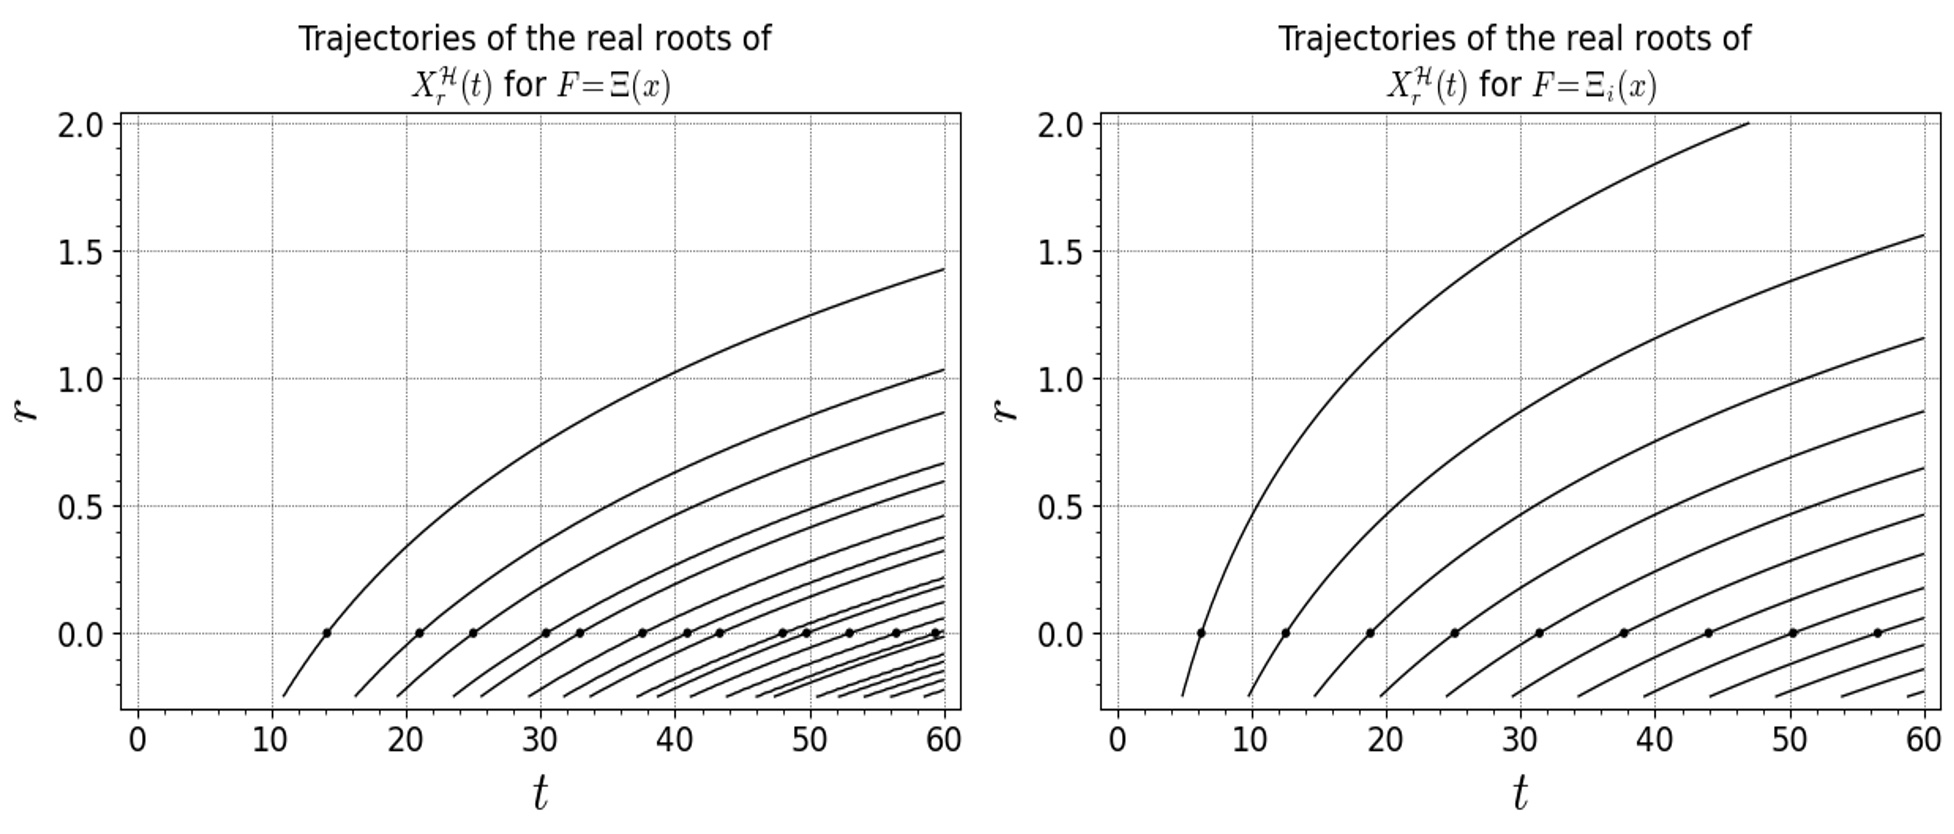
\includegraphics[width=1\linewidth]{HermiteFlowdouble.jpeg}
  \caption{The graphs show the Poisson flows of the Hermite polynomial expansions for $\Xi(t)$ (left) and $\Xi_i(t)$ (right). We know these flows are the transformation of the Pólya de Bruijn flow, i.e.: $X^\mathcal{H}_r(t) \verifiedeq\Xi_{\frac{\exp(-r)^2-1}{4}} (\exp(-r)\,t)$. Since the mapping $\exp(-r), r > 0$ can now only cover the domain $\lambda > 0$ we don't expect any collisions to show up in these Hermite flows (unless the RH is false somewhere high up).}
  \label{fig:flowH1}
\end{figure}

\pagebreak
\noindent\fbox{\begin{minipage}{\textwidth}
\begin{align}
  \textbf{Poisson}&\textbf{ Flow for the Generalised Laguerre polynomials} \notag \\
  L^{a}_n(x) &\defeq \frac{(\alpha+1)_n}{n!}\, {}_1F_1(-n, a+1,x) \\
  M_n(a) &\defeq \frac{\Gamma(\alpha+1+n)}{n!} \\
  w(x,a) &\defeq \mathrm{e}^{-x}\,x^a\\
  f_n(a) &\verifiedeq \frac{\Gamma\left(n+a+1\right)}{\Gamma(a+1)^2\,n!} \\
  -n\,y(x) &\verifiedeq x\,y''(x)+(\alpha+1-x)\,y'(x) \\
  X^{\mathcal{L}\,(d)}_r(t,a) &\verifiedeq \frac{a}{(a)_{d+1}}\,\sum_{n=0}^\infty \gamma_n(a)\,(-n)_d\,{}_1F_1\left(d-n, a+d+1,t\right)\,\exp(-r)^n \\ 
  \gamma_n(a) &\verifiedeq f_n(a)\int_{0^+}^{\infty} F(x)\,w(x,a)\,{}_1F_1\left(-n, a+1,x\right)\,\mathrm{d}x \\
  \sum_{n=0}^\infty \gamma_n(a) &\verifiedeq \Xi(0) \\
  \frac{\mathrm{d}}{\mathrm{d} r} z_k(r)&\verifiedeq-2\,z_k(r)\,\sum_{j \ne k}^{'} \frac{1}{z_k(r)-z_j(r)} -(\alpha+1-z_k(r))\\
  \frac{\mathrm{d}}{\mathrm{d} r} z_k(0)&\verifiedeq 2-(\alpha+1-2\,k\,\pi) \quad \text{when } F=\Xi_i
\end{align}
\end{minipage}}
\begin{figure}[H]
  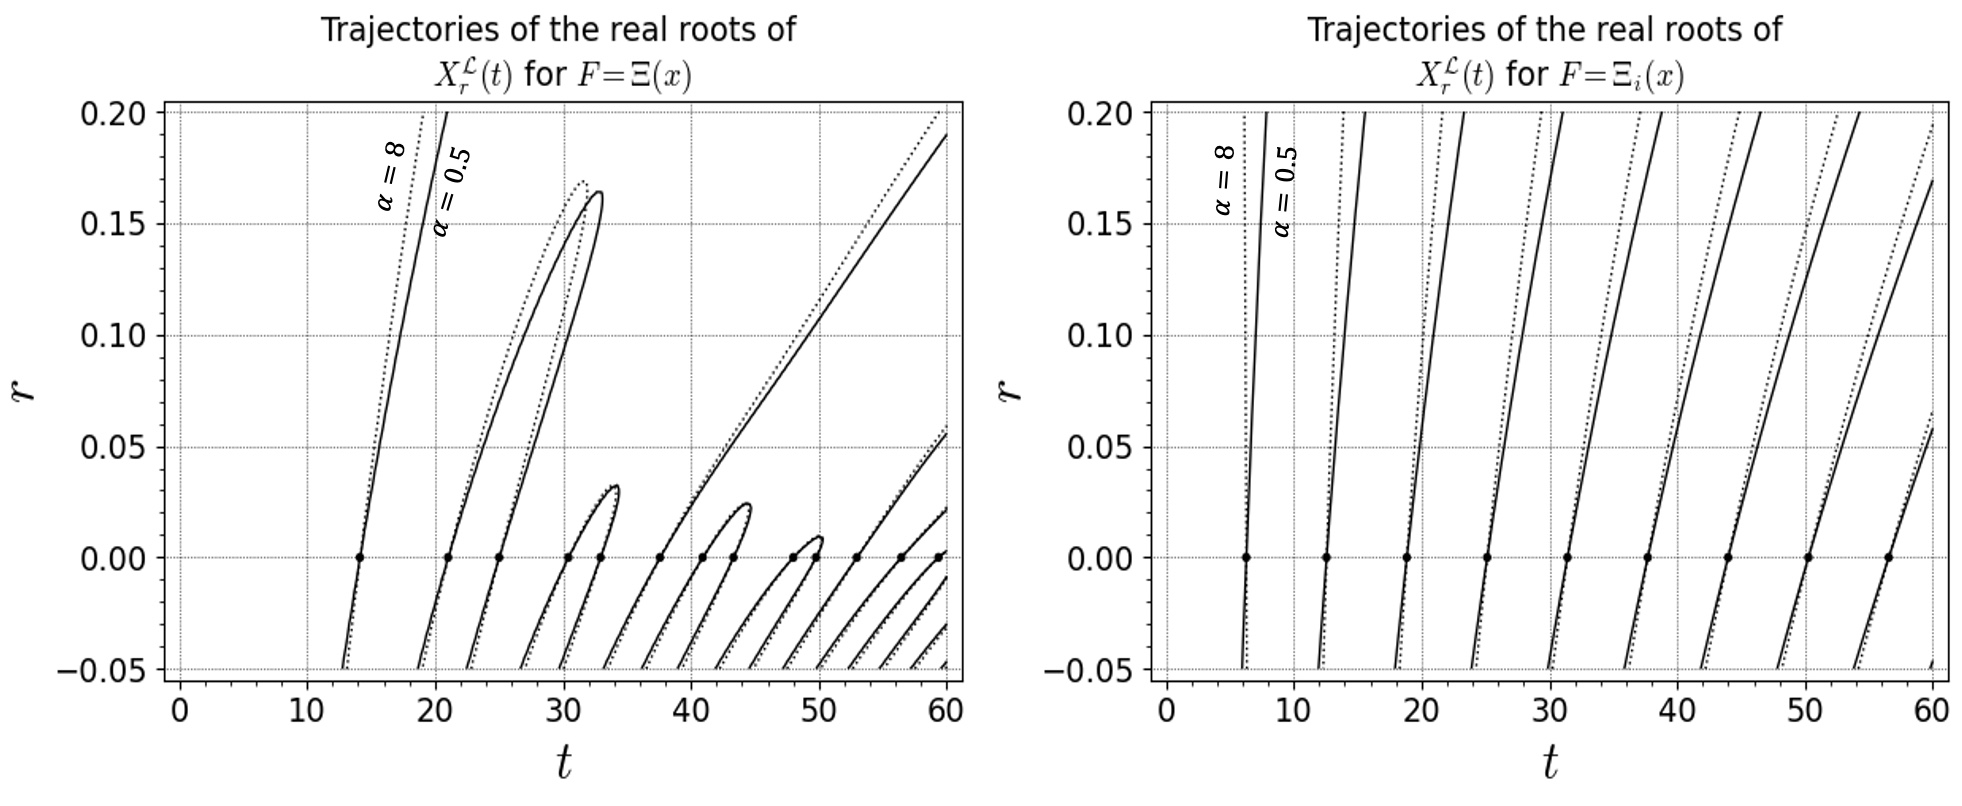
\includegraphics[width=1\linewidth]{LaguerreFlowdouble.jpeg}
  \caption{The graphs show the Poisson flows of the Generalised Laguerre polynomial expansions for $\Xi(t)$ (left) and $\Xi_i(t)$ (right). We show the flow for the parameters $\alpha = 0.5, \alpha = 8$. A change of a parameter induces a rotation around $r=0$. For $\alpha < 0$ the rotation is clock wise, $\alpha > 0$ goes counter clockwise. It would interesting to learn more about extreme rotations $\alpha \rightarrow \pm \infty$. We see similar patterns as in the Pólya-De Bruijn flow, however these cannot be connected in a similar fashion as the Hermite polynomials. When $r$ decreases the flows line up horizontally into an arithmetic progression.}
  \label{fig:flowL}
\end{figure}
\pagebreak
\noindent\fbox{\begin{minipage}{\textwidth}
\begin{align}
  \textbf{Poisson}&\textbf{ Flow for the Bessel $y_n$ polynomials} \notag \\
  y_n(x,a) &\defeq {}_2F_0\left(-n, n+a+1,[],-\frac{x}{2}\right) \\
  M_n(a) &\defeq -\frac{2^{a+1}\,\Gamma(-n-a)\,n!}{2n+a+1}\\
  w_x(a) &\defeq \mathrm{e}^{-\frac{2}{x}}\,x^a \\
  f_n(a) &\verifiedeq -\frac{\left(2n+a+1\right)}{2^{a+1}\,\Gamma(-n-a)\,n!} \\
  -n\,(n+a+1)\,y(x) &\verifiedeq -x^2\,y''(x)-\big((a+2)\,x+2\big)\,y'(x) \\ \label{besPDE}
  X^{\mathcal{B}\,(d)}_r(t,a) &\verifiedeq \frac{(-1)^d}{2^d}\sum_{n=0}^\infty \gamma_n(a)\frac{(n+a)_{d+1}(-n)_d}{n+a}{}_2F_0\left([d-n, n+a+d+1],[],-\frac{t}{2}\right)\exp\left(-r(n+a+1)\right)^n \\ \label{besflow}
  \gamma_n(a) &\verifiedeq f_n(a)\,\int_{0^+}^{\infty} F(x)\,w_x(a)\,{}_2F_0\left([-n, n+a+1],[],\frac{-x}{2}\right)\,\mathrm{d}x \\
  \sum_{n=0}^\infty \gamma_n(a) &\verifiedeq \Xi(0) \\
  \frac{\mathrm{d}}{\mathrm{d} r} z_k(r)&\verifiedeq 2\,z_k(r)^2\,\sum_{j \ne k}^{'} \frac{1}{z_k(r)-z_j(r)} + \big((a+2)\,z_k(r)+2\big)\\
  \frac{\mathrm{d}}{\mathrm{d} r} z_k(0)&\verifiedeq -2\,(2\,k\,\pi)+ \big((a+2)\,(2\,k\,\pi)+2\big) \quad \text{when } F=\Xi_i
\end{align}
\end{minipage}}
\begin{figure}[H]
  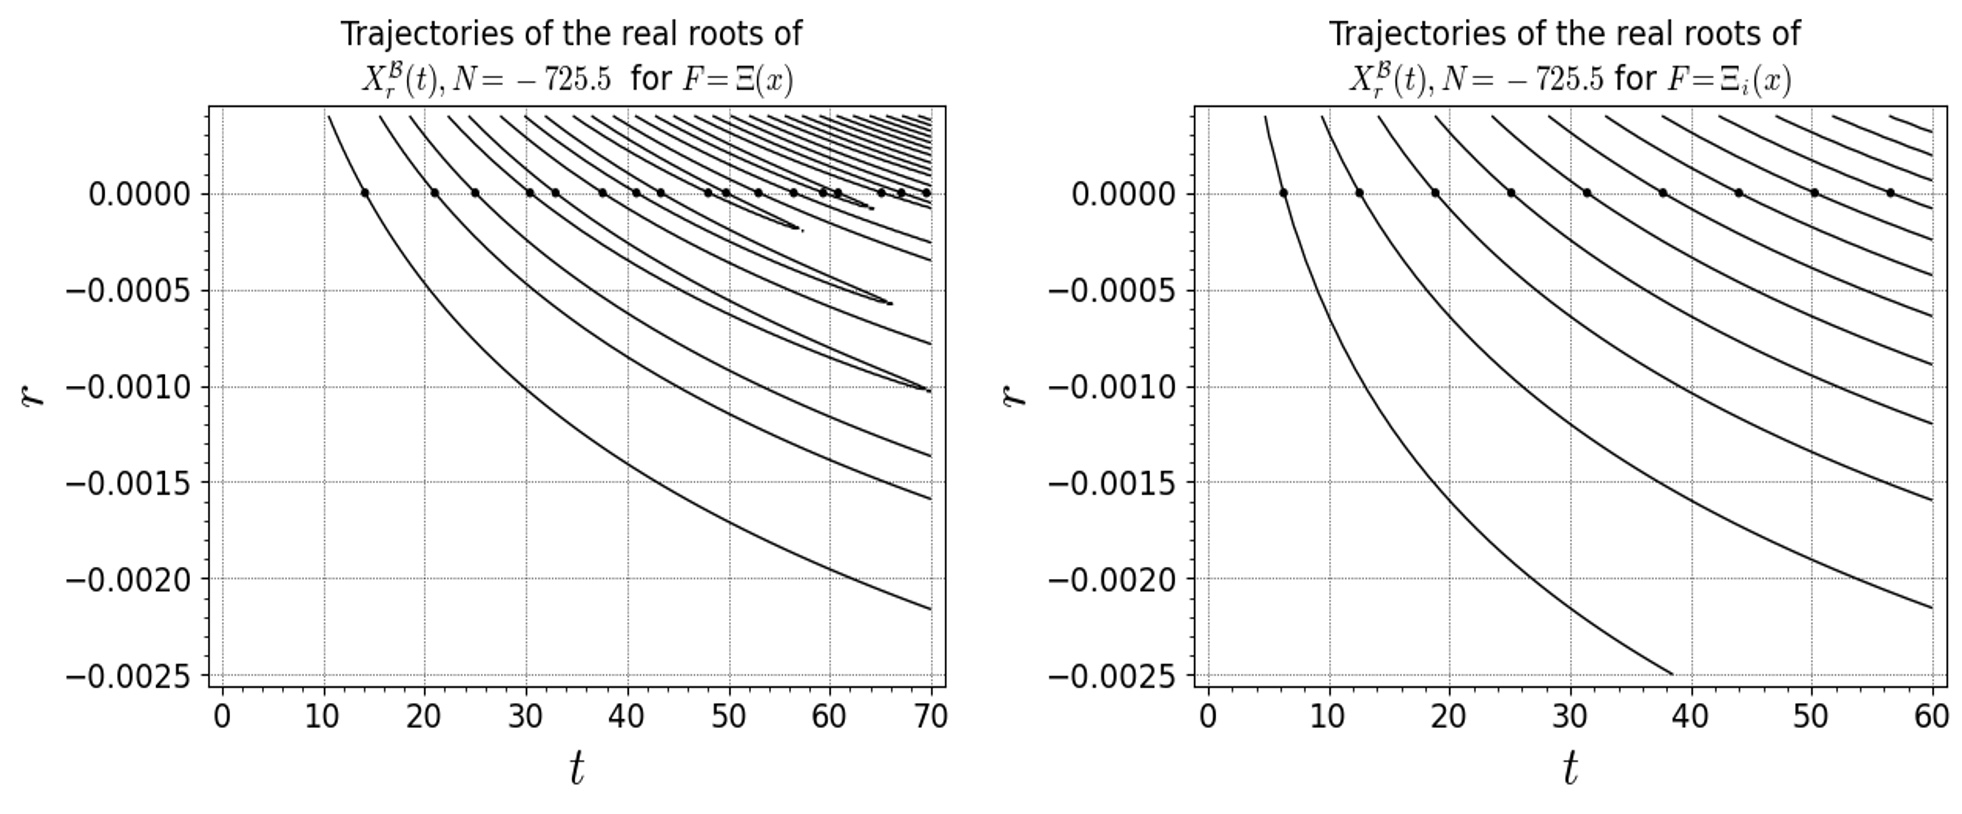
\includegraphics[width=1\linewidth]{BesselFlowdouble.jpeg}
  \caption{The graphs show the Poisson flows of the Bessel-$y$ polynomial expansions for $\Xi(t)$ (left) and $\Xi_i(t)$ (right) for a fixed set of parameters. The collisions show a similar pattern as in the Pólya-De Bruijn flow, but now flipped vertically and pushed to the right. When $r$ increases the flows line up horizontally into an arithmetic progression.}
  \label{fig:flowB}
\end{figure}
\pagebreak
\noindent\fbox{\begin{minipage}{\textwidth}
\begin{align}
  \textbf{Poisson}&\textbf{ Flow for the Meixner Pollaczek polynomials with $\Phi = \frac{\pi}{2}$} \notag \\
  P_n^{(\lambda)}\left(x, \frac{\pi}{2}\right) &\defeq i^n\,\frac{(2\lambda)_n}{n!}\,{}2F_1\left([-n, \lambda+i\,x],[2\lambda],2\right)\\
  M_n(\lambda) &\defeq \frac{2\,\pi\,\Gamma(n+2\lambda)}{2^{2\lambda}\,n!} \\
  w_x(\lambda) &\defeq \Gamma(\lambda+ix)\,\Gamma(\lambda-ix) \\
  f_n(\lambda) &\verifiedeq \frac{4^\lambda\,\Gamma(n+2\lambda)}{2\,\pi\,\Gamma(2\lambda)^2\,\Gamma(n+1)} \\
  -n\,y(x) &\verifiedeq -\frac12\,(\lambda-ix)\,y(x+i)+\lambda\,y(x)-\frac12\,(\lambda+ix)\,y(x-i) \\
  X^\mathcal{MP}_r(t,\lambda) &\verifiedeq \sum_{n=0}^\infty \gamma_{2n}(\lambda)\,{}_2F_1\left([-2n, \lambda+it],[2\lambda],2\right)\,\exp\left(-r\right)^{2n} \\ 
  \gamma_n(\lambda) &\verifiedeq f_n(\lambda)\,\int_{-\infty}^{\infty} F(x)\,w_x(\lambda)\,{}_2F_1\left([-n, \lambda+ix],[2\lambda],2\right)\,\mathrm{d}x \\
  \sum_{n=0}^\infty \gamma_n(\lambda) &\verifiedeq \Xi(i\lambda) \\
  \frac{\mathrm{d}}{\mathrm{d} r} z_k(r)&\verifiedeq  \left(\frac{\lambda-i\,z_k(r)}{2}\right)\,\prod_{j \ne k}^{'} \left(1+\frac{i}{z_k(r)-z_j(r)}\right)+\left(\frac{\lambda+i\,z_k(r)}{2}\right)\,\prod_{j \ne k}^{'} \left(1-\frac{i}{z_k(r)-z_j(r)}\right) \\
  \frac{\mathrm{d}}{\mathrm{d} r} z_k(0)&\verifiedeq \left(\frac{\lambda}{2}-k\,\pi\,i\right)\,ZP(k,i)+\left(\frac{\lambda}{2}+k\,\pi\,i\right)\,ZP(k,-i)\quad \text{when } F=\Xi_i 
\end{align}
\end{minipage}}
\begin{figure}[H]
  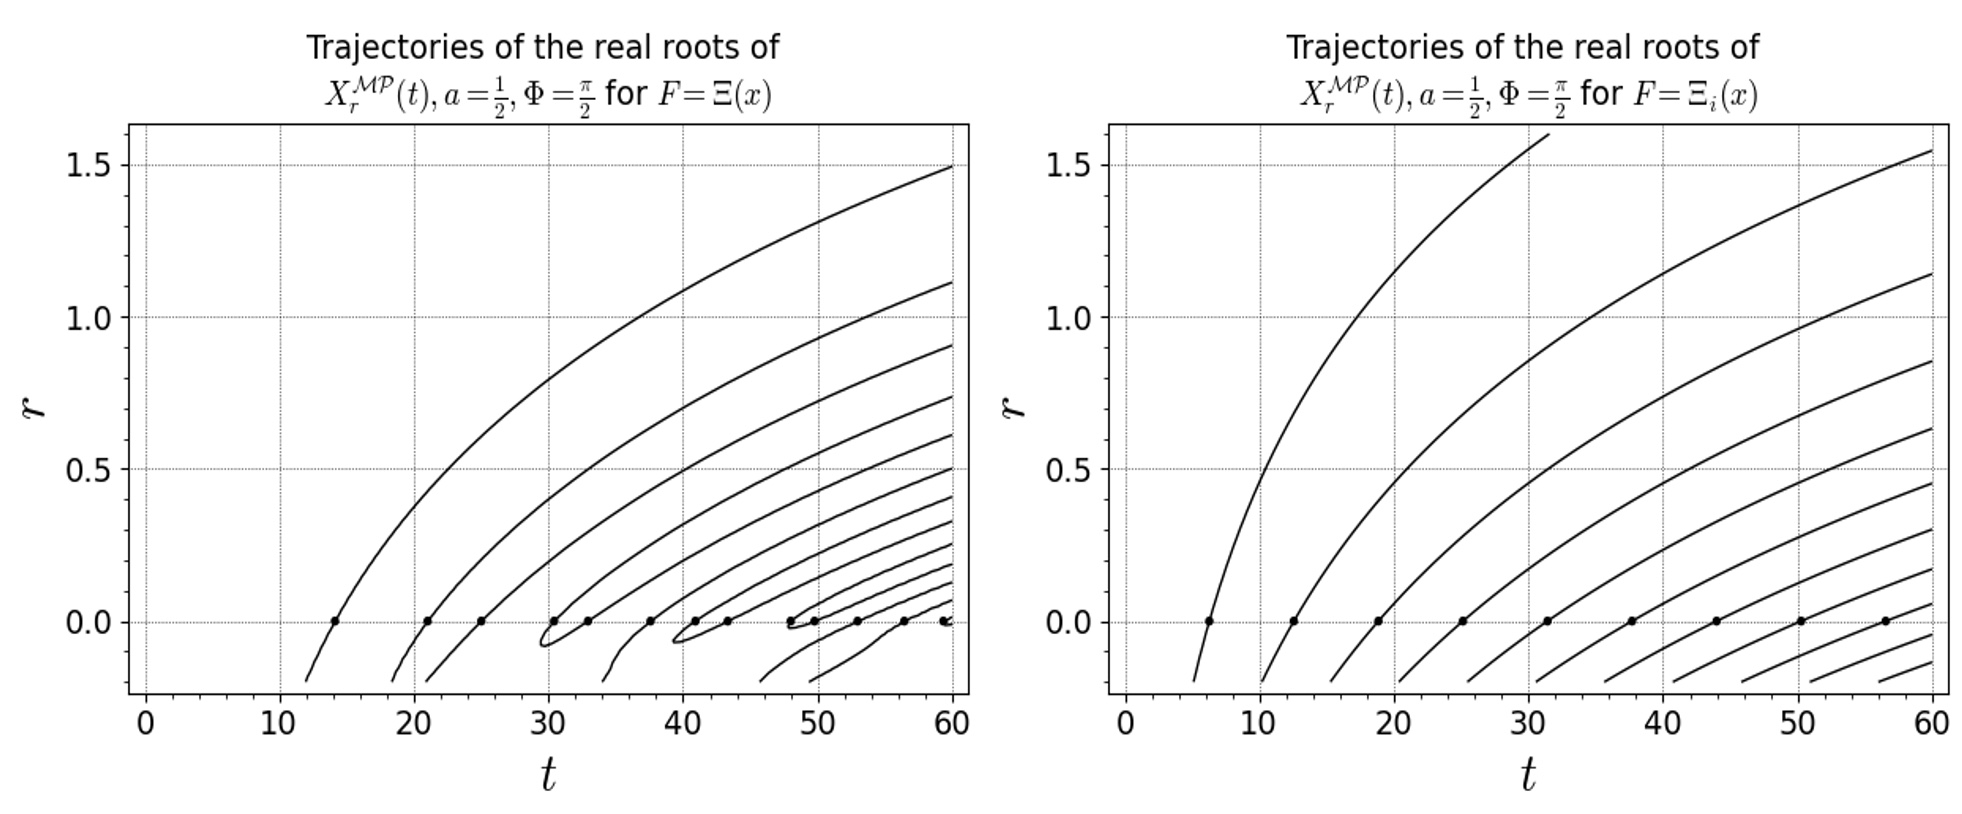
\includegraphics[width=1\linewidth]{MeixPollFlowdouble.jpeg}
  \caption{The graphs show the Poisson flows of the Meixner-Pollaczek polynomial expansions for $\Xi(t)$ (left) and $\Xi_i(t)$ (right) for a fixed set of parameters. The collisions seem to appear only at $r < 0$ and show a similar pattern as in the Pólya-De Bruijn flow, but now flipped vertically and pushed to the left. When $r$ increases the flows line up vertically into an arithmetic progression.}
  \label{fig:flowMP}
\end{figure}
\pagebreak
\noindent\fbox{\begin{minipage}{\textwidth}
\begin{align}
  \textbf{Poisson}&\textbf{ Flow for the Jacobi polynomials} \notag \\
  P_n(\alpha,\beta,x) &\defeq \frac{(\alpha+1)_n}{n!}\,{}_2F_1\left([-n, n+\alpha+\beta+1],[\alpha+1],\frac{1-x}{2}\right) \\
  M_n(\alpha,\beta) &\defeq \frac{2^{\alpha+\beta+1}}{2n+\alpha+\beta+1}\,\frac{\Gamma(n+\alpha+1)\,\Gamma(n+\beta+1)}{\Gamma(n+\alpha+\beta+1)\,n!}\\
  w_x(\alpha,\beta) &\defeq (1-x)^\alpha\,(1+x)^\beta \\
  f_n(\alpha,\beta) &\verifiedeq \frac{\Gamma(n+\alpha+1)\,\Gamma(n+\alpha+\beta+1)\,(2n+\alpha+\beta+1)}{2^{\alpha+\beta+1}\,\Gamma(\alpha+1)^2\,\Gamma(n+1)\,\Gamma(n+\beta+1)} \\
 -n\,(n+\alpha+\beta+1)\,y(x) &\verifiedeq (1-x^2)\,y''(x)+\big(\beta-\alpha-(\alpha+\beta+2)\,x\big)\,y'(x) \\
  X^{\mathcal{J}\,(d)}_r(t,\alpha,\beta) &\verifiedeq \frac{(-1)^d\,\alpha}{2^d\,(\alpha)_{d+1}}\,\sum_{n=0}^\infty \gamma_n(\alpha,\beta)\,\frac{(-n)_d\,(n+\alpha+\beta)_{d+1}}{n+\alpha+\beta}\\ &\times {}_2F_1\left([d-n, n+\alpha+\beta+d+1],[\alpha+d+1],\frac{1-t}{2}\right)\,\exp\left(-r(n+\alpha+\beta+1)\right)^n \\ 
  \gamma_n(\alpha,\beta) &\verifiedeq f_n(\alpha,\beta)\,\int_{-1^+}^{1^-} \Xi(x)\,w_x(\alpha,\beta)\,{}_2F_1\left([-n, n+\alpha+\beta+1],[\alpha+1],\frac{1-x}{2}\right)\,\mathrm{d}x \\
  \sum_{n=0}^\infty \gamma_n(\alpha,\beta) &\verifiedeq \Xi(1) \\
  \frac{\mathrm{d}}{\mathrm{d} r} z_k(r)&\verifiedeq -2\,(1-z_k(r)^2)\,\sum_{j \ne k}^{'} \frac{1}{z_k(r)-z_j(r)} - \big(\beta-\alpha-(\alpha+\beta+2)\,z_k(r)\big)\\
  \frac{\mathrm{d}}{\mathrm{d} r} z_k(0)&\verifiedeq 2\,\frac{(1-(2\,k\,\pi)^2)}{2\,k\,\pi}-\big(\beta-\alpha-(\alpha+\beta+2)\,(2\,k\,\pi)\big) \quad \text{when } F=\Xi_i
\end{align}
\end{minipage}}
\begin{figure}[H]
  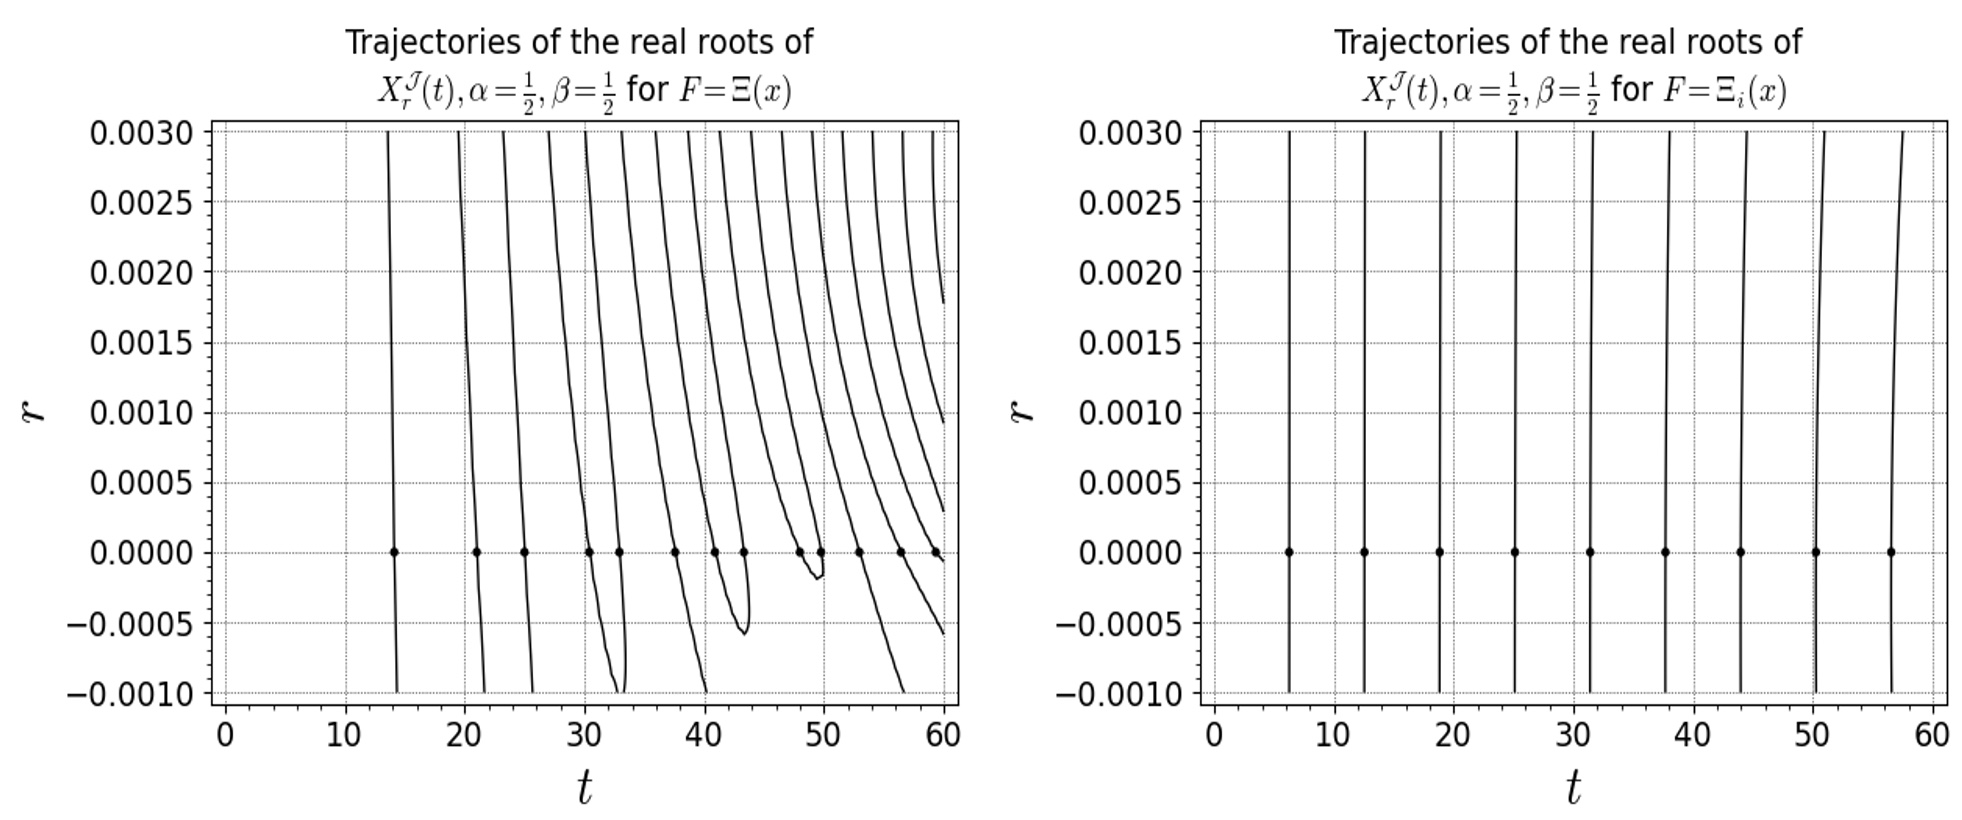
\includegraphics[width=1\linewidth]{JacobiFlowdouble.jpeg}
  \caption{The graphs show the Poisson flows of the Jacobi polynomial expansions for $\Xi(t)$ (left) and $\Xi_i(t)$ (right) for a fixed set of parameters. The collisions seem to appear only at $r < 0$ and show a similar pattern as in the Pólya-De Bruijn flow, but now flipped vertically. We made several runs with different sets of parameters, including those for the Gegenbauer/Ultraspherical ($\alpha=\beta=\lambda-\frac12$), Chebyshev ($\alpha=\beta=-\frac12$) and Legendre/Spherical ($\alpha=\beta=0$) polynomials, all with a very similar outcome. When $r$ increases the flows line up horizontally into an arithmetic progression.}
  \label{fig:flowJ}
\end{figure}
\pagebreak
\noindent\fbox{\begin{minipage}{\textwidth}
\begin{align}
  \textbf{Poisson}&\textbf{ Flow for the Pseudo Jacobi or Romanovski polynomials} \notag \\
  P_n(x,v,N) &\defeq \frac{(-2i)^n\,(-N+iv)_n}{(n-2N-1)_n}\,{}_2F_1\left([-n, n-2N-1],[-N+iv],\frac{1-ix}{2}\right)\\
  M_n(v,N) &\defeq \frac{2\pi\,\Gamma(2N+1-2n)\,\Gamma(2N+2-2n)\,2^{2n-2N-1}\,n!}{\Gamma(2N+2-n)\,|\Gamma(N+1-n+iv)|^2} \\
  w_x(v,N) &\defeq \left(1+x^2\right)^{-N-1}\,\mathrm{e}^{2a\,\arctan(x)}\\
  f_n(v,N) &\verifiedeq(-1)^n \frac{4^N\,(2N+1-2n)\,\Gamma(n-N+iv)^2\,|\Gamma(N+1-n+iv)|^2}{\pi\,n!\,\Gamma(2N+2-n)\,\Gamma(-N+iv)^2} \\
  -n\,(n-2N-1)\,y(x) &\verifiedeq -(1+x^2)\,y''(x)-2\,\big(v-Nx\big)\,y'(x) \\
  X^{\mathcal{PJ}\,(d)}_r(t,v,N) &\verifiedeq \frac{(-i)^d}{2^d\,(-N+iv)_d}\,\sum_{n=0}^\infty \gamma_n(v,N)\,(-n)_d\,(n-2N-1)_d\\ &\times{}_2F_1\left([d-n, n-2N-1+d],[d-N+iv],\frac{1-it}{2}\right)\,\exp\left(-r(n-2N-1)\right)^n \\ 
  \gamma_n(v,N) &\verifiedeq f_n(v,N)\,\int_{-\infty}^{\infty} \Xi(x)\,w_x(v,N)\,{}_2F_1\left([-n, n-2N-1],[-N+iv],\frac{1-ix}{2}\right)\,\mathrm{d}x \\
  \sum_{n=0}^\infty \Re(\gamma_n(v,N)) &\verifiedeq F(i), \,\,\sum_{n=0}^\infty \Im(\gamma_n(v,N)) = 0 \\
  \frac{\mathrm{d}}{\mathrm{d} r} z_k(r)&\verifiedeq 2\,(1+z_k(r)^2)\,\sum_{j \ne k}^{'} \frac{1}{z_k(r)-z_j(r)} + 2\,\big(v-N\,z_k(r)\big)\\
  \frac{\mathrm{d}}{\mathrm{d} r} z_k(0)&\verifiedeq -2\,\frac{(1+(2\,k\,\pi)^2)}{2\,k\,\pi}+ 2\,\big(v-N\,(2\,k\,\pi)\big) \quad \text{when } F=\Xi_i
\end{align}
\end{minipage}}
\begin{figure}[H]
  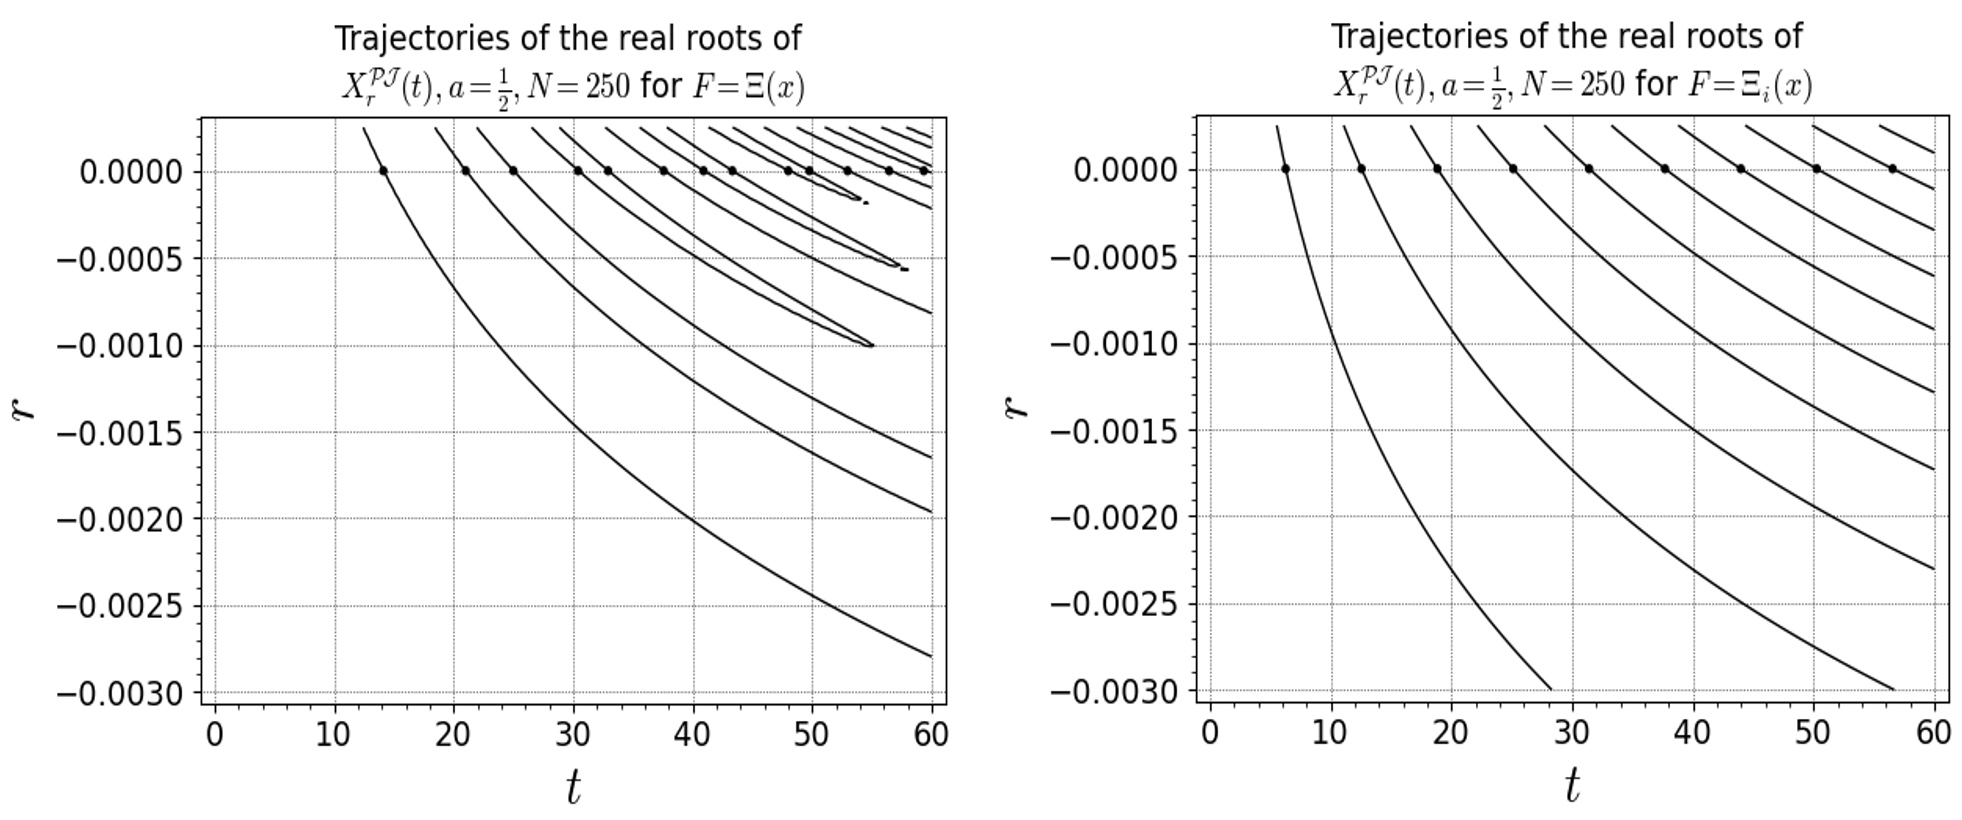
\includegraphics[width=1\linewidth]{PseudoJacobiFlowdouble.jpeg}
  \caption{The graphs show the Poisson flows of the Pseudo Jacobi polynomial expansions for $\Xi(t)$ (left) and $\Xi_i(t)$ (right) for a fixed set of parameters. The collisions seem to appear only at $r < 0$ and show a similar pattern as in the Pólya-De Bruijn flow, but now flipped vertically and pushed to the right. This graph looks very similar to the Bessel-$y$ expansion. When $r$ increases the flows line up horizontally into an arithmetic progression.}
  \label{fig:flowPJ}
\end{figure}
\pagebreak
\noindent\fbox{\begin{minipage}{\textwidth}
\begin{align}
  \textbf{Poisson}&\textbf{ Flow for the Continuous Dual Hahn polynomials} \notag \\
  S_n(x^2;a,b,c) &\defeq (a+b)_n(a+c)_n\, {}_3F_2([-n,a+ix, a- ix], [a+b, a+c], 1) \\
  M_n(a,b,c) &\defeq 2\pi\,n!\,\Gamma(n+a+b)\,\Gamma(n+a+c)\,\Gamma(n+b+c) \\
  w_x(a,b,c) &\defeq \left|\frac{\Gamma(a+ix)\,\Gamma(b+ix)\,\Gamma(c+ix)}{\Gamma(2ix)}\right|^2 \\
  f_n(a,b,c) &\verifiedeq \frac{\Gamma(n+a+b)\,\Gamma(n+a+c)}{2\,\pi\,\Gamma(a+b)^2\,\Gamma(a+c)^2\,n!\,\Gamma(n+b+c)} \\
  -n\,y(x) &\verifiedeq -B(x)\,y(x+i)+\left(B(x)+D(x)\right)\,y(x)-D(x)\,y(x-i) \\
  B(x)&\verifiedeq\frac{(a-ix)\,(b-ix)\,(c-ix)}{2ix\,(2ix-1)} \\
  D(x)&\verifiedeq\frac{(a+ix)\,(b+ix)\,(c+ix)}{(2ix\,(2ix+1)} \\
  X^\mathcal{CDH}_r(t,a,b,c) &\verifiedeq \sum_{n=0}^\infty \gamma_n(a,b,c)\,{}_3F_2\left([-n, a+it, a-it],[a+b,a+c],1\right)\,\exp\left(-r\right)^n \\ 
  \gamma_n(a,b,c) &\verifiedeq f_n(a,b,c)\,\int_{0}^{\infty} F(x)\,w_x(a,b,c)\,{}_3F_2\left([-n, a+ix, a-ix],[a+b,a+c],1\right)\,\mathrm{d}x \\
  \sum_{n=0}^\infty \gamma_n(a,b,c) &\verifiedeq \Xi(\pm ia) \\
  \frac{\mathrm{d}}{\mathrm{d} r} z_k(r)&\verifiedeq B\big(Z_k(r)\big)\,\prod_{j \ne k}^{'} \left(1+\frac{i}{z_k(r)-z_j(r)}\right)+D\big(Z_k(r)\big)\,\prod_{j \ne k}^{'} \left(1-\frac{i}{z_k(r)-z_j(r)}\right) \\
  \frac{\mathrm{d}}{\mathrm{d} r} z_k(0)&\verifiedeq B\big(2\,k\,\pi\big)\,ZP(k,i)+D\big(2\,k\,\pi)\,ZP(k,-i)\quad \text{when } F=\Xi_i 
\end{align}
\end{minipage}}
\begin{figure}[H]
  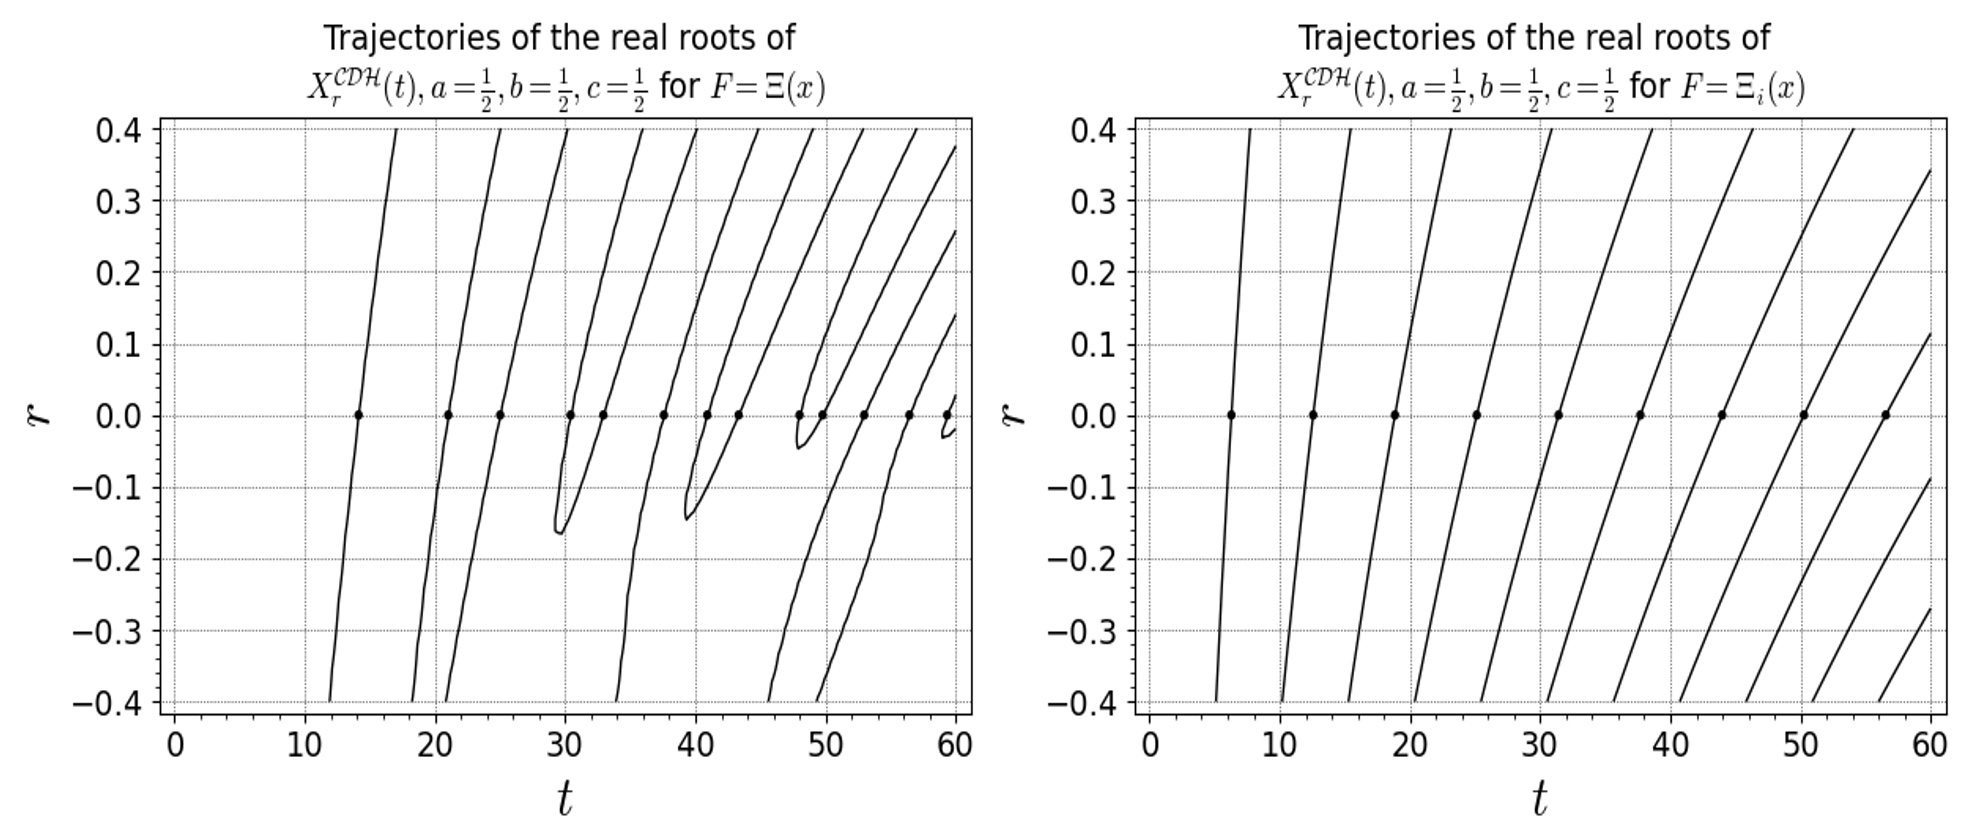
\includegraphics[width=1\linewidth]{ContDualHahnFlowdouble.jpeg}
  \caption{The graphs show the Poisson flows of the Continuous Dual Hahn polynomial expansions for $\Xi(t)$ (left) and $\Xi_i(t)$ (right) for a fixed set of parameters. The collisions seem to appear only at $r < 0$ and show a similar pattern as in the Pólya-De Bruijn flow, but now flipped vertically. When $r$ increases the flows line up horizontally into an arithmetic progression.}
  \label{fig:flowLCDH}
\end{figure}
\pagebreak
\noindent\fbox{\begin{minipage}{\textwidth}
\begin{align}
  \textbf{Poisson}&\textbf{ Flow for the Continuous Hahn polynomials} \notag \\
  \kappa_n &= n + a + b + c + d - 1 \\
  p_n(x,a,b,c,d) &\defeq i^n\,\frac{(a+c)_n\,(a+d)_n}{n!}\,{}_3F_2\left([-n, \kappa_n, a+ix],[a+c,a+d],1\right) \\
  M_n(a,b,c,d) &\defeq \frac{2\pi\,\Gamma(n+a+c)\,\Gamma(n+a+d)\,\Gamma(n+b+c)\,\Gamma(n+b+d)}{(n+\kappa_n)\,\Gamma(\kappa_n)\,n!} \\
  w_x(a,b,c,d) &\defeq \Gamma(a+ix)\,\Gamma(b+ix)\,\Gamma(c-ix),\Gamma(d-ix) \\
  f_n(a,b,c,d) &\verifiedeq \frac{\Gamma(n+a+c)\,\Gamma(n+a+d)\,\Gamma(\kappa_n)\,(n+\kappa_n)}{2\,\pi\,\Gamma(a+c)^2,\Gamma(a+d)^2\,\Gamma(n+1)\,\Gamma(n+b+c)\,\Gamma(n+b+d)} \\
 -n\,\kappa_n\,y(x) &\verifiedeq -B(x)\,y(x+i)+\left(B(x)+D(x)\right)\,y(x)-D(x)\,y(x-i) \\
  B(x)&\verifiedeq (c-ix)\,(d-ix) \\
  D(x)&\verifiedeq (a+ix)\,(b+ix) \\
  X^\mathcal{CH}_r(t,a,b,c,d) &\verifiedeq \sum_{n=0}^\infty \gamma_n(a,b,c,d)\,{}_3F_2\left([-n, \kappa_n, a+it],[a+c,a+d],1\right)\,\exp\left(-r\,\kappa_n\right)^n \\ 
  \gamma(n,a,b,c,d) &\verifiedeq f_n(a,b,c,d)\,\int_{0}^{\infty} F(x)\,w_x(a,b,c,d) {}_3F_2\left([-n, \kappa_n, a+ix],[a+c,a+d],1\right)\,\mathrm{d}x \\
  \sum_{n=0}^\infty \gamma_n(a,b,c,d) &= \Xi(ia) \\
  \frac{\mathrm{d}}{\mathrm{d} r} z_k(r)&\verifiedeq B\big(Z_k(r)\big)\,\prod_{j \ne k}^{'} \left(1+\frac{i}{z_k(r)-z_j(r)}\right)+D\big(Z_k(r)\big)\,\prod_{j \ne k}^{'} \left(1-\frac{i}{z_k(r)-z_j(r)}\right) \\
  \frac{\mathrm{d}}{\mathrm{d} r} z_k(0)&\verifiedeq B\big(2\,k\,\pi\big)\,ZP(k,i)+D\big(2\,k\,\pi)\,ZP(k,-i)\quad \text{when } F=\Xi_i 
\end{align}
\end{minipage}}
\begin{figure}[H]
  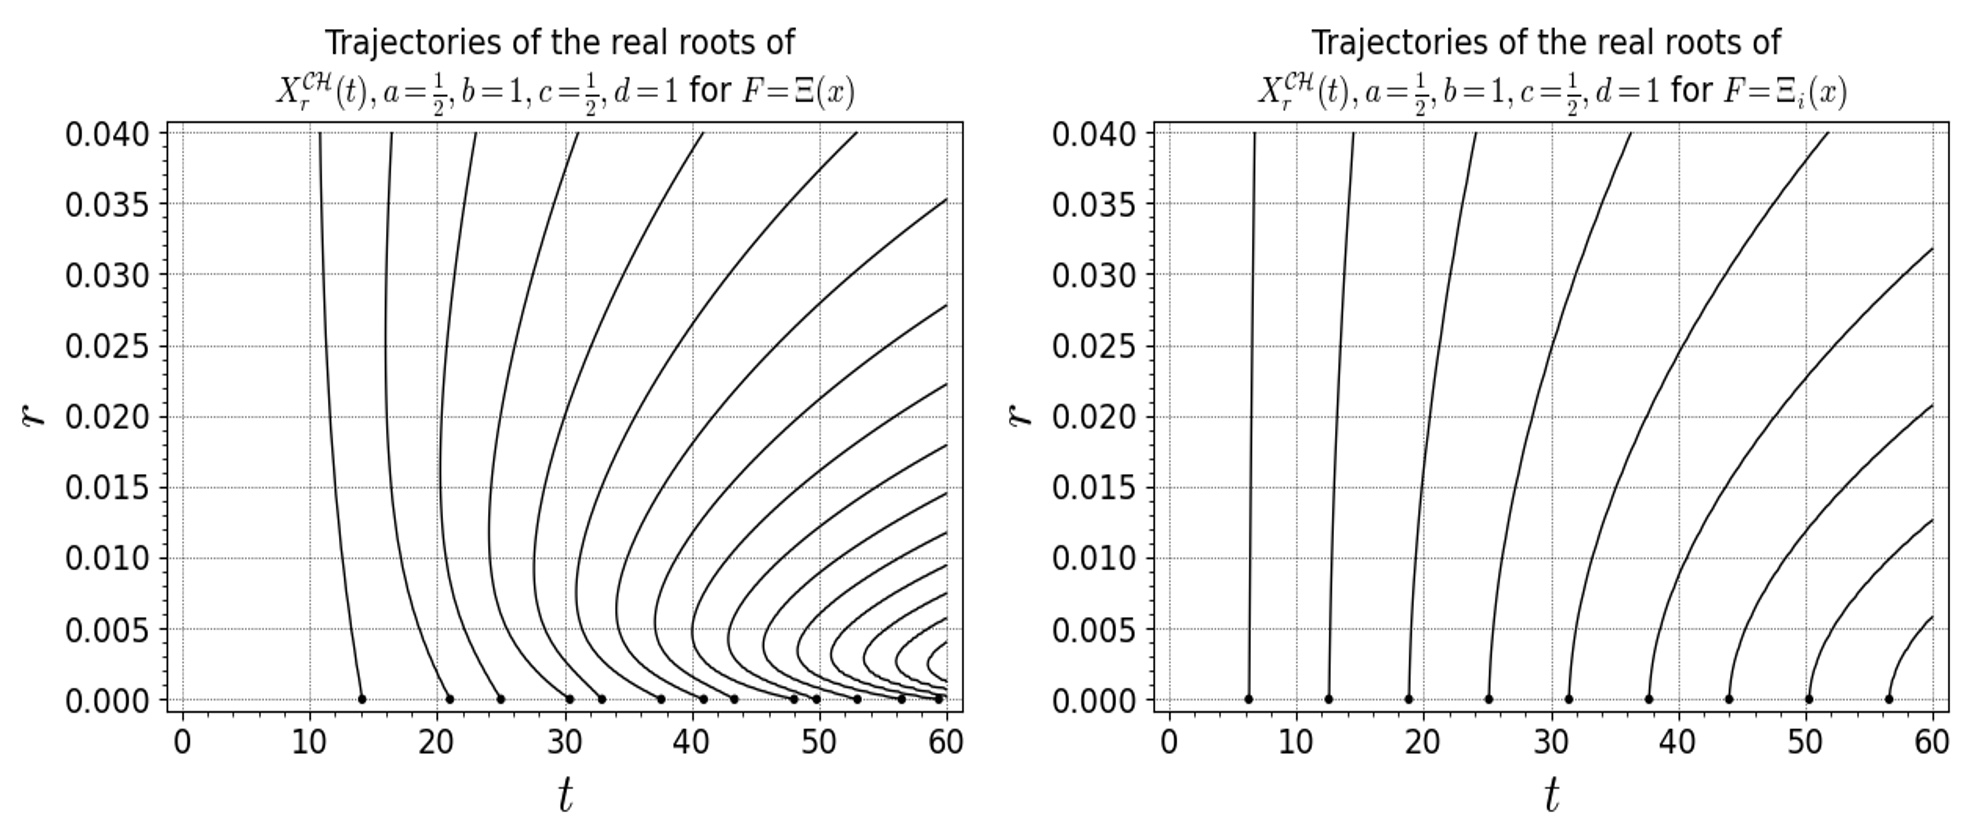
\includegraphics[width=1\linewidth]{ContHahnFlowdouble.jpeg}
  \caption{The graphs show the Poisson flows of the Continuous Hahn polynomial expansions for $\Xi(t)$ (left) and $\Xi_i(t)$ (right) for a fixed set of parameters. The domain $r < 0$ proved be invalid. When $t$ increases the flows line up vertically into an arithmetic progression. In theory this might be used to count the number of real zeros between $0 < r < R$ at point $T$, which should be equal to the number of zeros in the critical strip up till $T$.}
  \label{fig:flowCH}
\end{figure}
\pagebreak
\noindent\fbox{\begin{minipage}{\textwidth}
\begin{align}
  \textbf{Poisson}&\textbf{ Flow for the Wilson polynomials} \notag \\  
  \kappa_n &\defeq n + a + b + c + d - 1 \\
  W_n(y^2;a,b,c,d) &\defeq (a+b)_n(a+c)_n(a+d)_n {}_4F_3([-n, \kappa_n,a+iy, a- iy], [a+b, a+c, a+d], 1) \\
  M_n(a,b,c,d) &\defeq \frac{2\pi(\kappa_n)_nn!\Gamma(n+a+b)\Gamma(n+a+c)\Gamma(n+a+d)\Gamma(n+b+c)\Gamma(n+b+d)\Gamma(n+c+d)}{\Gamma(2n+a+b+c+d)}\\
  w_x(a,b,c,d) &\defeq \left|\frac{\Gamma(a+ix)\,\Gamma(b+ix)\,\Gamma(c+ix)\,\,\Gamma(d+ix)}{\Gamma(2ix)}\right|^2 \\
  f_n(a,b,c,d) &\verifiedeq \frac{(a+b)_n^2\,(a+c)_n^2\,(a+d)_n^2\,\Gamma(2n+a+b+c+d)}{2\pi\,(\kappa_n)_n\Gamma(n+a+b)\Gamma(n+a+c)\Gamma(n+a+d)n!\Gamma(n+b+c)\Gamma(n+b+d)\Gamma(n+c+d)}\\
  -n\,\kappa_n\,y(x) &\verifiedeq -B(x)\,y(x+i)+\left(B(x)+D(x)\right)\,y(x)-D(x)\,y(x-i) \\ \label{wildde}
  B(x)&\verifiedeq \frac{(a-ix)\,(b-ix)\,(c-ix)\,(d-ix)}{2ix\,(2ix-1)} \\
  D(x)&\verifiedeq \frac{(a+ix)\,(b+ix)\,(c+ix)\,(d+ix)}{(2ix\,(2ix+1)} \\
  X^\mathcal{W}_r(t,a,b,c,d) &\verifiedeq \sum_{n=0}^\infty \gamma_n(a,b,c,d)\,{}_4F_3\left(\left[-n, \kappa_n,a+it, a- it\right], \left[a+b, a+c, a+d\right], 1\right)\,\exp\left(-r\,\kappa_n\right)^n \\ \label{wilflow}
  \gamma(n,a,b,c,d) &\verifiedeq f_n(a,b,c,d)\int_{0}^{\infty} F(x)\,w_x(){}_4F_3\left(\left[-n, \kappa_n,a+ix, a- ix\right], \left[a+b, a+c, a+d\right], 1\right)\,\mathrm{d}x \\
  \sum_{n=0}^\infty \gamma_n(a,b,c,d) &\verifiedeq \Xi(\pm ia) \\
  \frac{\mathrm{d}}{\mathrm{d} r} z_k(r)&\verifiedeq B\big(Z_k(r)\big)\,\prod_{j \ne k}^{'} \left(1+\frac{i}{z_k(r)-z_j(r)}\right)+D\big(Z_k(r)\big)\,\prod_{j \ne k}^{'} \left(1-\frac{i}{z_k(r)-z_j(r)}\right) \\
  \frac{\mathrm{d}}{\mathrm{d} r} z_k(0)&\verifiedeq B\big(2\,k\,\pi\big)\,ZP(k,i)+D\big(2\,k\,\pi)\,ZP(k,-i)\quad \text{when } F=\Xi_i 
\end{align}
\end{minipage}}
\begin{figure}[H]
  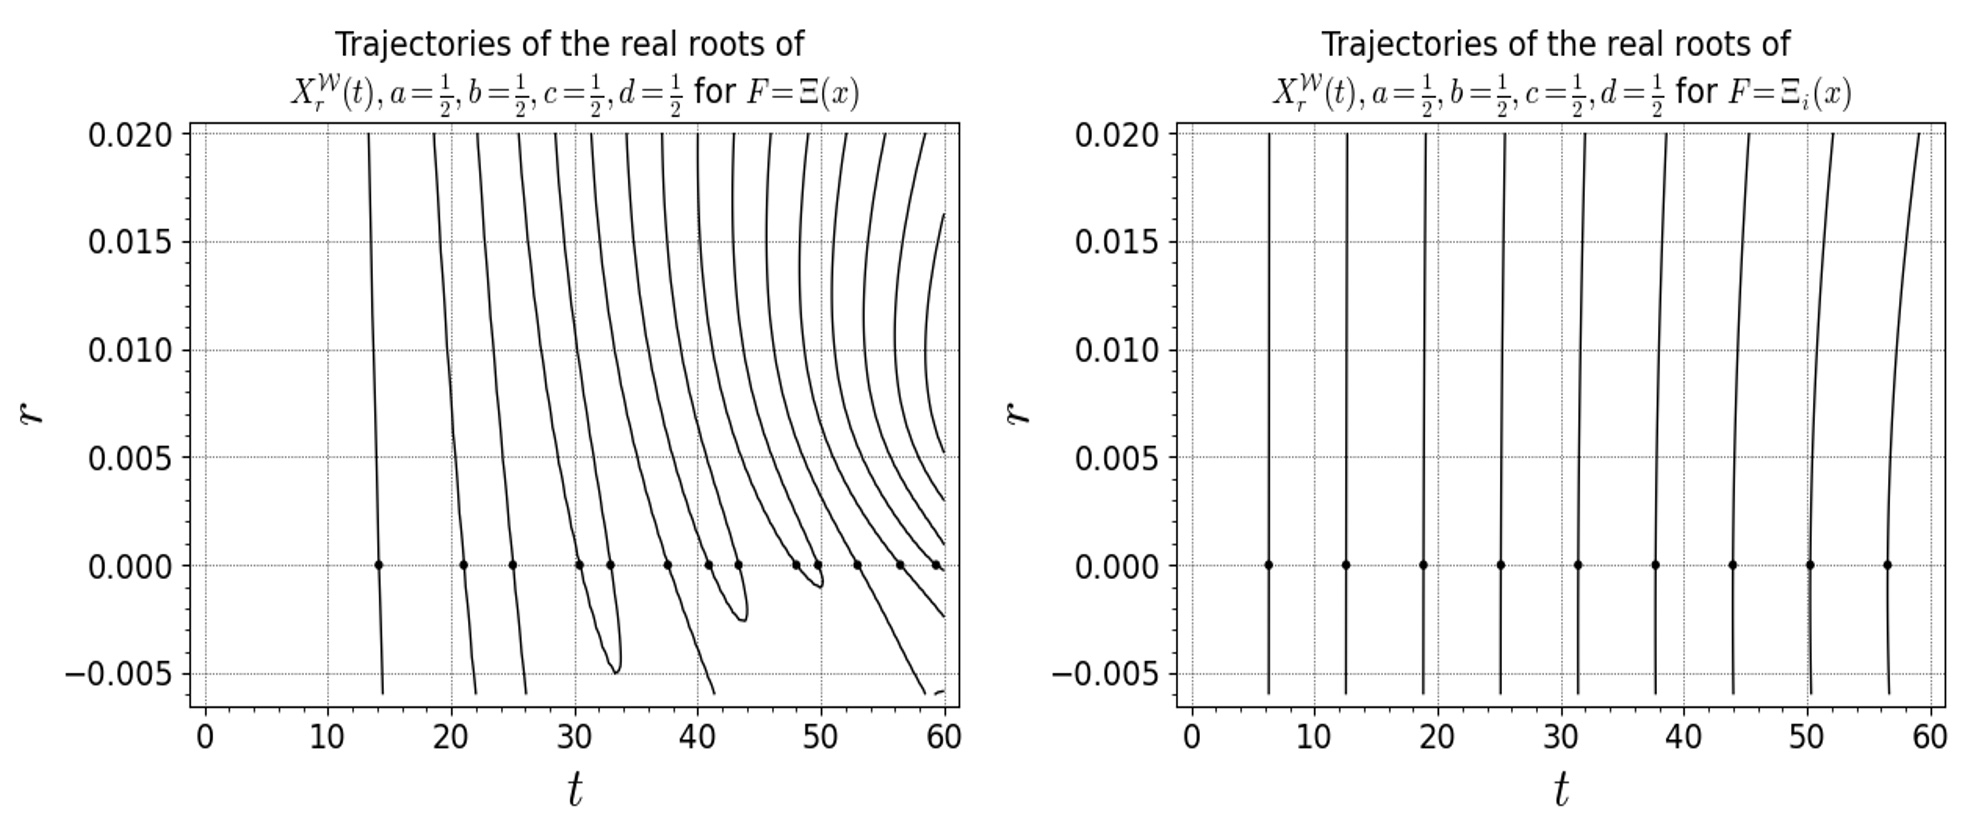
\includegraphics[width=1\linewidth]{WilsonFlowdouble.jpeg}
  \caption{The graphs show the Poisson flows of the Wilson polynomial expansions for $\Xi(t)$ (left) and $\Xi_i(t)$ (right) for a fixed set of parameters. The collisions seem to appear only at $r < 0$ and show a similar pattern as in the Pólya-De Bruijn flow, but now flipped vertically. When $t$ increases the flows line up vertically into an arithmetic progression in the domain $r > 0$.}
  \label{fig:flowW2}
\end{figure}
\end{small}
\pagebreak

\renewcommand{\theequation}{B.\arabic{equation}}
\setcounter{equation}{0}
\section{A list of alternatives for the coefficients of various Riemann $\Xi-$function expansions}\label{specexpansions}

There appears to be only a limited set of orthogonal polynomials whose generating function(s) can be directly linked to the kernel of the Fourier cosine transform of $\Xi(t)$ (or variants thereof). The table below is a simplified version of our findings in which we only show the integral part of the coefficients that we found. Their derivations can be found in the sections below. It is intriguing how the expansions of $\Xi(t)$ seem to be become infeasible beyond the Continuous Hahn family (the Continuous Dual Hahn and Wilson family expansions of $\Xi(t)$ are a bit "naughty"). 

\noindent\fbox{\begin{minipage}{\textwidth}
\begin{table}[H]
  \begin{center}
    \caption{Simplified coefficients for specific expansions}
    \label{tab:tablecoeff}
    \begin{tabular}{l|l|c|} 
      Polynomial family & Integral part of the coefficient $\gamma_n$ & Expands:\\
      \hline
      Hermite & $\displaystyle \int_{-\infty}^{\infty} \Phi(x)\,x^n\,\e^{-x^2/4}\, \mathrm{d}x $  &$\Xi(t)$ \\  
      Generalised Laguerre $\left(\alpha\right)$ & $\displaystyle  \int_{-\infty}^{\infty} \Phi(x)\,\left(\frac{ix}{ix+1}\right)^n\,\left(\frac{1}{ix+1}\right)^{\alpha+1}\,\mathrm{d}x $  &$\Xi(t)$ \\
      Meixner Pollaczek $\left(\lambda, \frac{\pi}{2}\right)$ & $\displaystyle \int_{-\infty}^{\infty} \Phi(x)\,\tanh\,\left(\frac{x}{2}\right)^n\,\frac{\textrm{e}^{\lambda\,x}}{(\textrm{e}^x+1)^{2\lambda}}\,\mathrm{d}x $  &$\Xi(t)$ \\ 
      Continuous Hahn $\left(\frac{a}{2},\frac{a+1}{2},\frac{a}{2},\frac{a+1}{2}\right)$ & $\displaystyle \int_{-\infty}^{\infty} \Phi(x)\,\tanh\left(\frac{x}{4}\right)^{n}\,\frac{\mathrm{e}^{ax/2}}{\left(\mathrm{e}^{x/2}+1\right)^{2a}}\,\mathrm{d}x  $  &$\Xi(t)$ \\   
      Continuous Hahn $\left(a,a,a,a\right)$ & $\displaystyle \int_{-\infty}^{\infty} \Phi(x)\,\tanh\left(\frac{x}{2}\right)^{n}\,\frac{\mathrm{e}^{ax}}{(\mathrm{e}^x+1)^{2a}}\,h_n(x,a)\, \mathrm{d}x$  &$\Xi(t)$ \\                  
      Continuous Dual Hahn $\left(a,0,\frac12\right)$ & $\displaystyle \int_{0}^{\infty} \Phi(x)\,\tanh\left(\frac{x}{2}\right)^{2n}\,\frac{\mathrm{e}^{ax}}{(\mathrm{e}^x+1)^{2a}}\,\mathrm{d}x $  &$\Xi(t)$ \\
      Continuous Dual Hahn $\left(a,1,\frac12\right)$ & $\displaystyle \int_{0}^\infty \Phi(x)\,\tanh\left(\frac{x}{2}\right)^{2n+1}\, \frac{x\,\mathrm{e}^{ax}}{(\mathrm{e}^x+1)^{2a}}\, \mathrm{d}x $  &$\Xi'(t)/t $ \\ 
      Wilson $\left(\frac{a}{2},\frac{a+1}{2},0,\frac12\right)$ & $\displaystyle \int_{0}^\infty \Phi(x)\,\tanh\left(\frac{x}{4}\right)^{2n}\,\frac{\mathrm{e}^{ax/2}}{\left(\mathrm{e}^{x/2}+1\right)^{2a}} \, \mathrm{d}x $  &$\Xi(t)$ \\
      Wilson $\left(\frac{a}{2},\frac{a+1}{2},\frac12,1\right)$ & $\displaystyle \int_{0}^\infty \Phi(x)\,\tanh\left(\frac{x}{4}\right)^{2n+1}\,\frac{x\,\mathrm{e}^{ax/2}}{\left(\mathrm{e}^{x/2}+1\right)^{2a}} \, \mathrm{d}x $  &$\Xi'(t)/t $ \\  
      Wilson $\left(\frac12,0,\frac12,0\right)$ & $\displaystyle \int_{0}^\infty \Phi(x)\,\tanh\left(\frac{x}{4}\right)^{2n}\, \mathrm{d}x $  &$\Xi(0) + \Xi(t)$ \\    
      Wilson $\left(\frac12,1,\frac12,1\right)$ & $\displaystyle \int_{0}^\infty \Phi(x)\,\tanh\left(\frac{x}{4}\right)^{2n+2}\, \mathrm{d}x $  &$\left(\Xi(0)-\Xi(t)\right)/t^2 $ \\          
    \end{tabular}
  \end{center}
\end{table}

where $\displaystyle h_n(x,a) \defeq {}_2F_1\left(\left[a+\frac{n}{2}, a+\frac{n+1}{2}\right],\left[2a+n+\frac12\right],\tanh\left(\frac{x}{2}\right)^2\right)$ and $\Phi(x)$ is defined in table (\ref{tab:tablefunc}).
\end{minipage}}

\begin{proposition}
The coefficients of the Laguerre polynomial expansion of $\Xi(x)$ can also be written into the simpler form: 
\begin{align}
\gamma_n(\alpha) &\verifiedeq \frac{(\alpha+1)_n}{\Gamma(a+1)\,n!}\,\int_{0^+}^{\infty} \Xi(x)\,\mathrm{e}^{-x}\,x^a\,{}_1F_1(-n,a+1,x)\,\mathrm{d}x \\
\gamma_n(\alpha) &\verifiedeq \frac{(\alpha+1)_n}{n!}\,\int_{-\infty}^{\infty} \Phi(x)\,\left(\frac{ix}{ix+1}\right)^n\,\left(\frac{1}{ix+1}\right)^{a+1}\,\mathrm{d}x
\end{align}
\end{proposition}
\begin{proof}
We start from the definition of the generalised Laguerre polynomial family:
\begin{equation}
 L^{\alpha}_n(t) \defeq \frac{(\alpha+1)_n}{n!}\, {}_1F_1(-n, \alpha+1,t) 
\end{equation}
Take its generating function and apply the mapping $x \mapsto \dfrac{ix}{1+ix}$:
\begin{align}
 \sum_{n=0}^\infty L^{\alpha}_n(t)\, x^n &\verifiedeq \frac{1}{(1-x)^{\alpha+1}}\,\exp\left(-\frac{tx}{1-x}\right) \qquad |x| < 1 \\
 \sum_{n=0}^\infty L^{\alpha}_n(t)\,\left(\frac{ix}{1+ix}\right)^n &\verifiedeq \textrm{e}^{-itx}\,\left(\frac{1}{1+xi} \right)^{-\alpha-1} \qquad |x| \in \mathbb{R}
\end{align}
Our target integral representation of $\Xi(t) = \Xi(-t)$ is:
\begin{align}
 \Xi(t) &\verifiedeq \int_{-\infty}^\infty \Phi(x)\,\textrm{e}^{-itx}\, \mathrm{d}x \\
 & \verifiedeq \int_{-\infty}^\infty \Phi(x)\,\textrm{e}^{-itx}\,\left(\frac{1}{1+xi} \right)^{-\alpha-1}\,\left(\frac{1}{1+xi} \right)^{\alpha+1} \, \mathrm{d}x \\
 & \verifiedeq \int_{-\infty}^\infty \Phi(x)\,\left( \sum_{n=0}^\infty L^{\alpha}_n(t)\,\left(\frac{ix}{1+ix}\right)^n\right)\,\left(\frac{1}{1+xi} \right)^{\alpha+1} \, \mathrm{d}x \\
  &\verifiedeq \sum_{n=0}^\infty L^{\alpha}_n(t)\,\int_{-\infty}^\infty \Phi(x)\,\left(\frac{ix}{1+ix}\right)^n\,\left(\frac{1}{1+xi} \right)^{\alpha+1}\, \mathrm{d}x
\end{align}
where $\Phi(x)$ is defined in table (\ref{tab:tablefunc}). The result follows after splitting up the polynomial into a leading and a hypergeometric factor.
\end{proof}

\begin{proposition}
The coefficients of the Meixner Pollaczek polynomial expansion of $\Xi(x)$ can also be written into the simpler form:   
\begin{align}
\gamma_n(\lambda) &\verifiedeq \frac{4^\lambda}{\pi}\,\frac{(2\lambda)_n}{\Gamma(2\lambda)\,n!}\,\int_{0}^{\infty} \Xi(x)\,\Gamma(\lambda+ix)\,\Gamma(\lambda-ix)\,{}_2F_1([-n,\lambda+ix],[2\lambda],2)\,\mathrm{d}x \\
\gamma_n(\lambda) &\verifiedeq 4^\lambda\,\frac{(2\lambda)_n}{n!}\,\int_{-\infty}^{\infty} \Phi(x)\,\tanh\,\left(\frac{x}{2}\right)^n\,\frac{\textrm{e}^{\lambda\,x}}{(\textrm{e}^x+1)^{2\lambda}}\,\mathrm{d}x
\end{align}
\end{proposition}
\begin{proof}
We start from the definition of the Meixner Pollaczek polynomials:
\begin{equation}
  P_n^{(\lambda)}\left(t,\frac{\pi}{2}\right) \defeq i^n\,\frac{(2\lambda)_n}{n!}\,{}2F_1\left([-n, \lambda+i\,t],[2\lambda],2\right)
\end{equation}
Take its generating function and apply the mapping: $x \mapsto i\,\dfrac{\textrm{e}^x-1}{\textrm{e}^x+1}$:
\begin{align}
 \sum_{n=0}^\infty P_n^{(\lambda)}\left(t,\frac{\pi}{2}\right)\,x^n &\verifiedeq (1-i\,x)^{-\lambda+i\,t}\,(1+i\,x)^{-\lambda-i\,t} \qquad |x| < 1 \\
 \sum_{n=0}^\infty P_n^{(\lambda)}\left(t,\frac{\pi}{2}\right)\,\left(i\,\frac{\textrm{e}^x-1}{\textrm{e}^x+1}\right)^n &\verifiedeq \textrm{e}^{-itx}\,4^{-\lambda}\, \textrm{e}^{-\lambda\,x}\,(\textrm{e}^x+1)^{2\lambda} \qquad |x| \in \mathbb{R}
\end{align}

Our target integral representation of $\Xi(t) = \Xi(-t)$ is:
\begin{align}
 \Xi(t) &\verifiedeq \int_{-\infty}^\infty \Phi(x)\,\textrm{e}^{-itx}\, \mathrm{d}x \\
 &\verifiedeq 4^\lambda \int_{-\infty}^\infty \Phi(x)\,\textrm{e}^{-itx}\,4^{-\lambda}\, \textrm{e}^{-\lambda\,x}\,(\textrm{e}^x+1)^{2\lambda}\,\frac{\textrm{e}^{\lambda\,x}}{(\textrm{e}^x+1)^{2\lambda}} \,\mathrm{d}x \\
 &\verifiedeq 4^\lambda \int_{-\infty}^\infty \Phi(x)\,\left(\sum_{n=0}^\infty i^n\,P_n^{(\lambda)}\left(t,\frac{\pi}{2}\right)\,\left(\frac{\textrm{e}^x-1}{\textrm{e}^x+1}\right)^n\right)\,\frac{\textrm{e}^{\lambda\,x}}{(\textrm{e}^x+1)^{2\lambda}} \, \mathrm{d}x \\
 &\verifiedeq 4^\lambda \sum_{n=0}^\infty i^n\,P_n^{(\lambda)}\left(t,\frac{\pi}{2}\right)\,\int_{-\infty}^\infty \Phi(x)\,\tanh\left(\frac{x}{2}\right)^n\,\frac{\textrm{e}^{\lambda\,x}}{(\textrm{e}^x+1)^{2\lambda}}\, \mathrm{d}x \label{meixner}
\end{align}
where $\Phi(x)$ is defined in table (\ref{tab:tablefunc}). The result follows after splitting up the polynomial into a leading and a hypergeometric factor.
\end{proof}

\begin{proposition}
The coefficients of the Continuous Hahn polynomial expansion of $\Xi(x)$ with parameters $\frac{a}{2}, \frac{a+1}{2},\frac{a}{2},\frac{a+1}{2}$, can also be written into the simpler form ($w_x$ is the weight function): 
\begin{align}
\gamma_n(a) &\verifiedeq \frac{16^a}{4\pi^2}\,\frac{(2a)_n}{\Gamma(2a)\,n!}\,\int_{-\infty}^{\infty} \Xi(x)\,w_x\left(\frac{a}{2},\frac{a+1}{2},\frac{a}{2},\frac{a+1}{2}\right)\,{}_3F_2\left(\left[-n,2a+n,\frac{a}{2}+ix\right],\left[a,a+\frac12\right],1\right)\,\mathrm{d}x \\
\gamma_n(a) &\verifiedeq (-1)^n\,4^a\,\frac{(2a)_n}{n!}\,\int_{-\infty}^{\infty} \Phi(x)\,\tanh\left(\frac{x}{4}\right)^{n}\,\frac{\mathrm{e}^{ax/2}}{\left(\mathrm{e}^{x/2}+1\right)^{2a}}\,\mathrm{d}x
\end{align}
\end{proposition}
\begin{proof}
We start from the definition of the Continuous Hahn family of polynomials:
\begin{align}
 p_n(t;a,b,c,d) &\defeq i^n\,\frac{(a+c)_n(a+d)_n}{n!}\, {}_3F_2([-n, n+ a+b+c+d-1,a+it], [a+c, a+d], 1) \notag
\end{align}
and use the relation between the Continuous Hahn and Meixner Pollaczek families (see eq. 30 in \cite{koesup}):
\begin{align}
 p_n\left(x;a,a+\frac12,a,a+\frac12\right) \verifiedeq \frac{(2a)_n\,\left(2a+\frac12\right)_n}{(4a)_n}\, P_n^{(2a)}\left(2x,\frac{\pi}{2}\right)
\end{align}

Applying this relation to \ref{meixner} yields:

\begin{align}
 \Xi(t)\verifiedeq 4^a \sum_{n=0}^\infty i^n\,p_n\left(t;\frac{a}{2},\frac{a+1}{2},\frac{a}{2},\frac{a+1}{2}\right)\,\frac{(2a)_n}{(a)_n\,\left(a+\frac12\right)_n}\,\int_{-\infty}^\infty \Phi(x)\,\tanh\left(\frac{x}{4}\right)^n\,\frac{\textrm{e}^{ax/2}}{(\textrm{e}^{x/2}+1)^{2a}}\, \mathrm{d}x
\end{align}
where $\Phi(x)$ is defined in table (\ref{tab:tablefunc}). The result follows after splitting the polynomial into its leading and hypergeometric factors.
\end{proof}

\begin{proposition}
The coefficients of the Continuous Hahn polynomial expansion of $\Xi(x)$ with all parameters $a,a,a,a$ equal, $a \in \mathbb{R}, a \ne \frac14$, can alternatively be written as (note $w_x(a,a,a,a)$ is the weight): 
\begin{align}
\gamma_n &\verifiedeq \frac{(2n+4a-1)\,\Gamma(n+4a-1)}{2\pi\,\Gamma(2a)^4\,n!}\,\int_{-\infty}^{\infty} \Xi(x)\,w_x\left(a,a,a,a)\,{}_3F_2([-n,n+4a-1,a+ix],[2a,2a],a\right)\,\mathrm{d}x \\
\gamma_n &\verifiedeq \frac{(-1)^n\,2^{2a-n}\,(2a)_n\,(4a-1)_n}{n!\,\left(2a-\frac12\right)_n}\int_{-\infty}^{\infty} \Phi(x)\tanh\left(\frac{x}{2}\right)^{n}\,\frac{\mathrm{e}^{ax}}{(\mathrm{e}^x+1)^{2a}}{}_2F_1\left(\left[a+\frac{n}{2}, a+\frac{n+1}{2}\right],\left[2a+n+\frac12\right],\tanh\left(\frac{x}{2}\right)^2\right)\mathrm{d}x \notag
\end{align}
\end{proposition}
\begin{proof}
We start from some finite sum definitions of the Meixner-Pollaczek and the Continuous Hahn polynomials that are obtained by just writing their hypergeometric function as a finite sum:

\begin{align}
 f_n(x,a) &\defeq P_n^{a)}\left(t,\frac{\pi}{2}\right) \defeq i^n\,\frac{(2a)_n}{n!}\,{}2F_1\left([-n, a+i\,t],[2a],2\right) \\
 &= (-i)^n\,\sum_{m=0}^n\,\frac{2^m\,\Gamma(2a+n)}{(n-m)!\,\Gamma(2a+m)}\,\binom{-a+ix}{m} \\
 g_n(x,a) &\defeq p_n(t;a,a,a,a) \defeq i^n\,\frac{(4a-1)_n}{n!}\, {}_3F_2([-n, n+ 4a-1,a+it], [2a, 2a], 1) \\
 &\defeq (-i)^n\,\sum_{m=0}^n\,\frac{(4a-1)_{n+m}}{(n-m)!\,(2a)_m^2}\,\binom{-a+ix}{m}
\end{align}

Next, we express $f_n(x,a)$ into $g_n(x,a)$ and vice versa:

\begin{align}
g_n(x,a) &\verifiedeq \sum_{k=0}^{\lfloor n/2\rfloor} \frac{2^{n-2k}\,\left(2a-\frac12\right)_{n-k}}{k!\,(2a)_{n-2k}}\,f_{n-2k}(x,a) \\
f_n(x,a) &\verifiedeq \frac{(2a)_n}{2^n\,\left(2a-\frac12\right)_{n+1}}\,\sum_{k=0}^{\lfloor n/2\rfloor} (-1)^k\,\left(n-2k+2a-\frac12\right)\,\binom{n+2a-\frac12}{k}\,g_{n-2k}(x,a)
\end{align}

The proof of the above relations follows the same steps as the proof for the special case $a=\frac34$ in appendix (A.6) of Romik's extended paper \cite{rom}. The steps of the proof are not repeated here, since the only difference is that in equation (A.45) we have to start with $p=n-m$ and $q=m+2a-\frac32$ and in equation (A.49) we have to use $N\verifiedeq n + 2a - \frac12, m\verifiedeq m +2a-\frac32$ (note there is an innocent typo in (A.49), the last factor in the RHS should be $2^{n-m-1}$ instead of $2^{n-m+1}$).

The second equation above allows us to equate the generating functions of $f_n(x,a)$ and $g_n(x,a)$ as follows:
\begin{align}
 \sum_{n=0}^\infty f_n(t,a)\,x^n &\verifiedeq \sum_{n=0}^\infty \frac{(2a)_n}{2^n\,\left(2a-\frac12\right)_n}\,{}_2F_1\left(\left[a+\frac{n}{2}, a+\frac{n+1}{2}\right],\left[2a+n+\frac12\right],-x^2\right) \,g_n(t,a)\,x^n \\
 &\verifiedeq (1-ix)^{-a+it}\,(1+ix)^{-a-it})
\end{align}
where the derivation towards the hypergeometric function again follows the exact same steps as in Romik's paper (Lemma 5.7. and its proof on p50). 

We apply the mapping $x \mapsto \left(i\,\dfrac{\textrm{e}^{x}-1}{\textrm{e}^{x}+1}\right)$ to make it converge for $x \in \mathbb{R}$ and set $$h(x,n,a) \defeq {}_2F_1\left(\left[a+\frac{n}{2}, a+\frac{n+1}{2}\right],\left[2a+n+\frac12\right],\left(\dfrac{\textrm{e}^{x}-1}{\textrm{e}^{x}+1}\right)^2\right)$$

We obtain:
\begin{align}
 \sum_{n=0}^\infty \frac{(2a)_n}{2^n\,\left(2a-\frac12\right)_n}\,h(x,n,a) \,g_n(t,a)\,\left(i\,\dfrac{\textrm{e}^{x}-1}{\textrm{e}^{x}+1}\right)^n \verifiedeq 4^{-a}\mathrm{e}^{itx}\mathrm{e}^{-ax}\left(\mathrm{e}^x+1\right)^{2a} 
\end{align}

Our target integral representation of $\Xi(t) = \Xi(-t)$ is:
\begin{align}
  \Xi(t)&\verifiedeq\int_{-\infty}^\infty \Phi(x)\,\mathrm{e}^{-ixt}\, \mathrm{d}x\\
  &\verifiedeq 4^a\, \int_{-\infty}^\infty \Phi(x)\,4^{-a}\mathrm{e}^{itx}\,\mathrm{e}^{-ax}\,\left(\mathrm{e}^x+1\right)^{2a}\,\frac{\mathrm{e}^{ax}}{\left(\mathrm{e}^x+1\right)^{2a}} \mathrm{d}x \\
   &\verifiedeq 4^a\,\int_{-\infty}^\infty \Phi(x)\, \left(\sum_{n=0}^\infty \frac{(2a)_n}{2^n\,\left(2a-\frac12\right)_n}\,h(x,n,a) \,g_n(t,a)\left(i\,\dfrac{\textrm{e}^{x}-1}{\textrm{e}^{x}+1}\right)^n\right)\,\frac{\mathrm{e}^{ax}}{\left(\mathrm{e}^x+1\right)^{2a}} \mathrm{d}x\\
   &\verifiedeq 4^a\, \sum_{n=0}^\infty i^n\,\frac{(2a)_n \,g_n(t,a)}{2^n\,\left(2a-\frac12\right)_n}\int_{-\infty}^\infty \Phi(x)\,\,h(x,n,a)\left(\dfrac{\textrm{e}^{x}-1}{\textrm{e}^{x}+1}\right)^n\,\frac{\mathrm{e}^{ax}}{\left(\mathrm{e}^x+1\right)^{2a}} \mathrm{d}x
\end{align}

where $\Phi(x)$ is defined in table (\ref{tab:tablefunc}). The result follows after splitting up the polynomial into a leading and a hypergeometric factor.
\end{proof}

\begin{proposition}
The coefficients of the Continuous Dual Hahn polynomial expansion of $\Xi(x)$ for parameters $a,0,\frac12$, can also be written into the following simpler form:   
\begin{align}
  \gamma_n(a) &\verifiedeq \frac{4^a}{4\,\pi^2}\,\frac{(2a)_{2n}}{\Gamma(2n+1)\,\Gamma(2a)}\,\int_{0}^{\infty} \Xi(x)\,w_x\left(a,0,\frac12\right)\,{}_3F_2\left([-n,a+ix,a-ix],\left[a,a+\frac12\right],1\right)\mathrm{d}x \\
  \gamma_n(a) &\verifiedeq 2\,4^a\,\frac{(a)_n\,\left(a+\frac12\right)_n}{\left(\frac12\right)_n\,n!}\,\int_{0}^{\infty} \Phi(x)\,\tanh\left(\frac{x}{2}\right)^{2n}\,\frac{\mathrm{e}^{ax}}{(\mathrm{e}^x+1)^{2a}}\,\mathrm{d}x
\end{align}
\end{proposition}
\begin{proof}
We start from the definition of the Continuous Dual Hahn family of polynomials:
\begin{equation}
 S_n(t^2;a,b,c) \defeq (a+b)_n(a+c)_n\, {}_3F_2([-n,a+it, a- it], [a+b, a+c], 1) 
\end{equation}

and take generating function (9.3.14) in \cite{koe} and set $a=a,b=0,c=\frac12$ (note that formally all parameters should be larger than $0$, however putting one to $0$ does work numerically), Using Mathematica we find:
\begin{align}
 \sum_{n=0}^\infty \frac{S_n(t^2;a,b,c)}{(b+c)_n\,n!}\, x^n &\verifiedeq (1-x)^{-a+it}\,{}_2F_1\left([b+it, c+it],[b+c], x\right) \\
\sum_{n=0}^\infty \frac{S_n\left(t^2;a,0,\frac12\right)}{\left(\frac12\right)_n\,n!}\,x^n&\verifiedeq \frac12\,(1-x)^{-a+it}\left((1-\sqrt{x})^{1-2(1/2+it)}+(1+\sqrt{x})^{1-2(1/2+it}\right)
\end{align}

We now apply the mapping $x \mapsto \left(\dfrac{\textrm{e}^{x}-1}{\textrm{e}^{x}+1}\right)^2$ which yields:
\begin{equation}
 \sum_{n=0}^\infty \frac{S_n\left(t^2;a,0,\frac12\right)}{\left(\frac12\right)_n\,n!}\, \left(\frac{\textrm{e}^{x}-1}{\textrm{e}^{x}+1}\right)^{2n} \verifiedeq \cos(tx)\,4^{-a}\,(\mathrm{e}^x+1)^{2a}\,\mathrm{e}^{-ax}
\end{equation}

Our target integral representation of $\Xi(t) = \Xi(-t)$ is:
\begin{align}
 \Xi(t) &\verifiedeq 2\,\int_{0}^\infty \Phi(x)\cos(tx)\, \mathrm{d}x \\
 &\verifiedeq 2\,4^a\,\int_{0}^\infty \Phi(x)\,\cos(tx)\,4^{-a}\,(\mathrm{e}^x+1)^{2a}\,\mathrm{e}^{-ax} \,\frac{\mathrm{e}^{ax}}{(\mathrm{e}^x+1)^{2a}} \mathrm{d}x \\
 &\verifiedeq 2\,4^a\,\int_{0}^\infty \Phi(x)\,\left(\sum_{n=0}^\infty \frac{S_n\left(t^2;a,0,\frac12\right)}{\left(\frac12\right)_n\,n!}\, \left(\frac{\textrm{e}^{x}-1}{\textrm{e}^{x}+1}\right)^{2n}\right)\,\frac{\mathrm{e}^{ax}}{(\mathrm{e}^x+1)^{2a}}\, \mathrm{d}x \\
 &\verifiedeq 2\,4^a\,\sum_{n=0}^\infty \frac{S_n\left(t^2;a,0,\frac12\right)}{\left(\frac12\right)_n\,n!}\,\int_{0}^{\infty} \Phi(x)\,\tanh\left(\frac{x}{2}\right)^{2n}\,\frac{\mathrm{e}^{ax}}{(\mathrm{e}^x+1)^{2a}}\,\mathrm{d}x \label{cdh0}
\end{align}
where $\Phi(x)$ is defined in table (\ref{tab:tablefunc}). The result follows after splitting up the polynomial into a leading and a hypergeometric factor.
\end{proof}

\begin{proposition}
The coefficients of the Continuous Dual Hahn polynomial expansion of $\Xi'(t)/t$ with parameters $(a,1,\frac12)$, can also be written into a simpler form (note $w_x$ is the weight):   
\begin{align}
 \gamma_n(a) &\verifiedeq -\frac{4^{a}}{\pi^2}\,\frac{\left(2a+1\right)_{2n}}{\Gamma(2n+2)\,\Gamma(2a+1)} \,\int_{0^+}^\infty \frac{\Xi'(x)}{x}\,w_x\left(a,1,\frac12\right)\,{}_3F_2\left([-n,a+ix,a-ix],\left[a+1,a+\frac12\right],1\right)\, \mathrm{d}x \\
 \gamma_n(a) &\verifiedeq -4^{a+1}\,\frac{\left(a+\frac12\right)_n\,(a+1)_n}{{\left(\frac32\right)_n\,n!}} \,\int_{0}^\infty \Phi(x)\,\tanh\left(\frac{x}{2}\right)^{2n+1}\, \frac{x\,\mathrm{e}^{ax}}{(\mathrm{e}^x+1)^{2a}}\, \mathrm{d}x \label{cdh1}
\end{align}
\end{proposition}
\begin{proof}
We start from the definition of the Continuous Dual Hahn family of polynomials:
\begin{equation}
 S_n(t^2;a,b,c) \defeq (a+b)_n(a+c)_n\, {}_3F_2([-n,a+it, a- it], [a+b, a+c], 1) 
\end{equation}

and take generating function (9.3.14) in \cite{koe} and set $a=a,b=1,c=\frac12$ and keep $a$ as a free parameter. Using Mathematica, we get:
\begin{align}
 \sum_{n=0}^\infty \frac{S_n(t^2;a,b,c)}{(b+c)_n\,n!}\, x^n &\verifiedeq (1-x)^{-a+it}\,{}_2F_1\left([b+it, c+it],[b+c] ;x\right) \\
\sum_{n=0}^\infty \frac{S_n\left(t^2;a,1,\frac12\right)}{\left(\frac32\right)_n\,n!}\,x^n&\verifiedeq (1-x)^{-a+it}\,\left(-i\,\frac{(1-\sqrt{x})^{-2it}-(1+\sqrt{x})^{-2it}}{4\,t\sqrt{x}}\right)
\end{align}

We now apply the mapping $x \mapsto \left(\dfrac{\textrm{e}^{x}-1}{\textrm{e}^{x}+1}\right)^2$ which yields:
\begin{equation}
 \sum_{n=0}^\infty \frac{S_n\left(t^2;a,1,\frac12\right)}{\left(\frac32\right)_n\,n!}\, \left(\frac{\textrm{e}^{x}-1}{\textrm{e}^{x}+1}\right)^{2n} \verifiedeq \frac{\mathrm{e}^{-ax}\,(\mathrm{e}^x+1)^{2a}}{2\,4^a\,t}\,\left(\frac{\textrm{e}^{x}+1}{\textrm{e}^{x}-1}\right)\,\sin(tx)
\end{equation}

Our target integral representation of $\Xi'(t) = -\Xi'(-t)$ is:
\begin{align}
 \Xi'(t) &\verifiedeq -2\,\int_{0}^\infty \Phi(x)\,x\sin(tx)\, \mathrm{d}x \\
 &\verifiedeq -4^{a+1}\,t\, \int_{0}^\infty \Phi(x)\,\frac{\mathrm{e}^{-ax}\,(\mathrm{e}^x+1)^{2a}}{2\,4^a\,t}\,\left(\frac{\textrm{e}^{x}+1}{\textrm{e}^{x}-1}\right)\,\sin(tx)\, \frac{x\,\mathrm{e}^{ax}}{(\mathrm{e}^x+1)^{2a}}\,\left(\frac{\textrm{e}^{x}-1}{\textrm{e}^{x}+1}\right) \mathrm{d}x \\
 &\verifiedeq -4^{a+1}\,t\, \int_{0}^\infty \Phi(x)\,\left(\sum_{n=0}^\infty \frac{S_n\left(t^2;a,1,\frac12\right)}{\left(\frac32\right)_n\,n!}\, \left(\frac{\textrm{e}^{x}-1}{\textrm{e}^{x}+1}\right)^{2n}\right)\, \frac{x\,\mathrm{e}^{ax}}{(\mathrm{e}^x+1)^{2a}}\,\left(\frac{\textrm{e}^{x}-1}{\textrm{e}^{x}+1}\right)\, \mathrm{d}x \\
 &\verifiedeq -4^{a+1}\,t\,\sum_{n=0}^\infty \frac{S_n\left(t^2;a,1,\frac12\right)}{\left(\frac32\right)_n\,n!}\, \int_{0}^\infty \Phi(x)\,\tanh\left(\frac{x}{2}\right)^{2n+1}\, \frac{x\,\mathrm{e}^{ax}}{(\mathrm{e}^x+1)^{2a}}\, \mathrm{d}x
\end{align}
where $\Phi(x)$ is defined in table (\ref{tab:tablefunc}). The result follows after splitting up the polynomial into a leading and a hypergeometric factor.
\end{proof}

\begin{proposition}
The coefficients of the Wilson polynomial expansion of $\Xi(t)$ with parameters $\frac{a}{2},\frac{a+1}{2},0,\frac12$, can also be written into the simpler form (note $w_x$ is the weight):   
\begin{align}
 \gamma_n(a) &\verifiedeq\frac{16^a}{8\pi^3}\,\frac{(2a)_{2n}}{\Gamma(2n+1)\,\Gamma(2a)}\,\int_{0}^\infty \Xi(x)\,w_x\left(\frac{a}{2},\frac{a+1}{2},0,\frac12\right) \,{}_4F_3\left(\left[-n,n+a,\frac{a}{2}+ix, \frac{a}{2}-ix\right],\left[a+\frac12,\frac{a}{2},\frac{a}{2}+\frac12\right],1\right) \mathrm{d}x \\
 \gamma_n(a) &\verifiedeq\frac{2^{2a+1}\,(2a)_{2n}}{(2n)!}\,\int_{0}^\infty \Phi(x)\,\tanh\left(\frac{x}{4}\right)^{2n}\,\frac{\mathrm{e}^{ax/2}}{\left(\mathrm{e}^{x/2}+1\right)^{2a}} \, \mathrm{d}x \notag
\end{align}
\end{proposition}
\begin{proof}
We start from the definition of the Wilson family of polynomials:
\begin{align}
 W_n(t^2;a,b,c,d) &\defeq (a+b)_n(a+c)_n(a+d)_n\, \\
  &\times\, {}_4F_3([-n, n+ a+b+c+d-1,a+it, a- it], [a+b, a+c, a+d], 1) \notag
\end{align}
and use the relation between the Wilson and Continuous Dual Hahn families (see eq. 25 in \cite{koesup}):
\begin{align}
 S_n\left(x;a,b,\frac12\right) \verifiedeq \frac{4^n}{(a+b+n)_n}\, W_n\left(\frac{x}{4};\frac{a}{2},\frac{a+1}{2},\frac{b}{2},\frac{b+1}{2}\right)
\end{align}
Applying this relation to \ref{cdh0} yields:
\begin{align}
  \Xi(t)\verifiedeq 2\,4^a\,\sum_{n=0}^\infty \frac{4^n\,W_n\left(t^2;\frac{a}{2},\frac{a+1}{2},0,\frac12\right)}{(a+n)_n\,\left(\frac12\right)_n\,n!}\,\int_{0}^{\infty} \Phi(x)\,\tanh\left(\frac{x}{4}\right)^{2n}\,\frac{\mathrm{e}^{ax/2}}{(\mathrm{e}^{x/2}+1)^{2a}}\,\mathrm{d}x
\end{align}
where $\Phi(x)$ is defined in table (\ref{tab:tablefunc}). The result follows after splitting the polynomial into its leading and hypergeometric factors.
\end{proof}

\begin{proposition}
The coefficients of the Wilson polynomial expansion of $\Xi'(t)/t$ with parameters $\frac{a}{2},\frac{a+1}{2},\frac12,1$, can also be written into the simpler form (note $w_x$ is the weight):   
\begin{align}
 \gamma_n(a) &\verifiedeq-\frac{2\,16^a}{\pi^3}\,\frac{(2a+1)_{2n}}{\Gamma(2n+2)\,\Gamma(2a+1)}\,\int_{0}^\infty \frac{\Xi'(x)}{x}\,w_x\left(\frac{a}{2},\frac{a+1}{2},\frac12,1\right) \,\\ &\qquad \times {}_4F_3\left(\left[-n,n+a+1,\frac{a}{2}+ix, \frac{a}{2}-ix\right],\left[a+\frac12,\frac{a}{2}+\frac12,\frac{a}{2}+1\right],1\right) \mathrm{d}x \notag \\
 \gamma_n(a) &\verifiedeq -8\,4^a\,\frac{(2a+1)_{2n}}{\Gamma(2n+2)}\,\int_{0}^\infty \Phi(x)\,\tanh\left(\frac{x}{4}\right)^{2n+1}\,\frac{x\,\mathrm{e}^{ax/2}}{\left(\mathrm{e}^{x/2}+1\right)^{2a}} \, \mathrm{d}x
\end{align}
\end{proposition}
\begin{proof}
We start from the definition of the Wilson family of polynomials:
\begin{align}
 W_n(t^2;a,b,c,d) &\defeq (a+b)_n(a+c)_n(a+d)_n\, \\
  &\times\, {}_4F_3([-n, n+ a+b+c+d-1,a+it, a- it], [a+b, a+c, a+d], 1) \notag
\end{align}
and use the relation between the Wilson and Continuous Dual Hahn families (see eq. 25 in \cite{koesup}):
\begin{align}
 S_n\left(x;a,b,\frac12\right) \verifiedeq \frac{4^n}{(a+b+n)_n}\, W_n\left(\frac{x}{4};\frac{a}{2},\frac{a+1}{2},\frac{b}{2},\frac{b+1}{2}\right)
\end{align}
Applying this relation to \ref{cdh1} yields:
\begin{align}
  \Xi'(t)\verifiedeq -8\,4^a\,t\,\sum_{n=0}^\infty \frac{4^n\,W_n\left(t^2;\frac{a}{2},\frac{a+1}{2},\frac12,1\right)}{(a+1+n)_n\,\left(\frac32\right)_n\,n!}\,\int_{0}^{\infty} \Phi(x)\,\tanh\left(\frac{x}{4}\right)^{2n+1}\,\frac{\mathrm{e}^{ax/2}}{(\mathrm{e}^{x/2}+1)^{2a}}\,\mathrm{d}x
\end{align}
where $\Phi(x)$ is defined in table (\ref{tab:tablefunc}). The result follows after splitting the polynomial into its leading and hypergeometric factors.
\end{proof}

\begin{proposition}
The coefficients of the Wilson polynomial expansion of $\Xi(0) +\Xi(t)$ with parameters $\frac12,0,\frac12,0$, can be written as:   
\begin{align}
\gamma_n &\verifiedeq 4\,\int_{0}^\infty \Phi(x)\,\tanh\left(\frac{x}{4}\right)^{2n}\, \mathrm{d}x \notag
\end{align}
\end{proposition}
\begin{proof}
We start from the definition of the Wilson family of polynomials:
\begin{align}
 W_n(t^2;a,b,c,d) &\defeq (a+b)_n(a+c)_n(a+d)_n\, \\
  &\times\, {}_4F_3([-n, n+ a+b+c+d-1,a+it, a- it], [a+b, a+c, a+d], 1) \notag
\end{align}
Its generating function valid for $|x| < 1$. We set $a=\frac12,b=0,c=\frac12,d=0$ and obtain a simpler form (note that formally all parameters should be larger than $0$, however putting two to $0$ does work numerically). Using Mathematica we find:
\begin{align}
 \sum_{n=0}^\infty \frac{W_n(t^2;a,b,c,d)}{(a+b)_n(c+d)_n\,n!}\, x^n &\verifiedeq {}_2F_1\left([a+it, b+it],[a+b] ;x\right)\,{}_2F_1\left(c-it, c-it,],[c+d],x\right) \\
 \sum_{n=0}^\infty \frac{W_n\left(t^2;\frac12,0,\frac12,0\right)}{\left(\frac12\right)_n\left(\frac12\right)_n\,n!}\,x^n&\verifiedeq \frac14\,\left((1-\sqrt{x})^{-2it}+(1+\sqrt{x})^{-2it}\right)\,\left((1-\sqrt{x})^{2it}+(1+\sqrt{x})^{2it}\right)
\end{align} 
We apply the mapping $x \mapsto \left(\dfrac{\textrm{e}^{\frac{x}{2}}-1}{\textrm{e}^{\frac{x}{2}}+1}\right)^2$ to make it converge for $x \in \mathbb{R}$ and obtain: 
\begin{align}
 &\sum_{n=0}^\infty \frac{W_n\left(t^2;\frac12,0,\frac12,0\right)}{\left(\frac12\right)_n\left(\frac12\right)_n\,n!}\, \left(\frac{\textrm{e}^{\frac{x}{2}}-1}{\textrm{e}^{\frac{x}{2}}+1}\right)^{2n} \verifiedeq \frac{\cos(tx)+1}{2}
\end{align}
Our target integral representation of $\Xi(t) = \Xi(-t)$ is:
\begin{align}
 \Xi(t) &\verifiedeq 2\,\int_{0}^\infty \Phi(x)\,\cos(t\,x)\, \mathrm{d}x \\
  &\verifiedeq -\Xi(0) +4\,\int_{0}^\infty \Phi(x)\, \frac{\cos(tx)+1}{2}  \mathrm{d}x\\
  &\verifiedeq -\Xi(0)+4\,\int_{0}^\infty \Phi(x)\,\left(\sum_{n=0}^\infty \frac{W_n\left(t^2;\frac12,0,\frac12,0\right)}{\left(\frac12\right)_n\left(\frac12\right)_n\,n!}\, \left(\frac{\textrm{e}^{\frac{x}{2}}-1}{\textrm{e}^{\frac{x}{2}}+1}\right)^{2n}\right) \mathrm{d}x \\
  &\verifiedeq -\Xi(0)+4\, \sum_{n=0}^\infty \frac{W_n\left(t^2;\frac12,0,\frac12,0\right)}{\left(\frac12\right)_n\left(\frac12\right)_n\,n!}\,\int_{0}^\infty \Phi(x)\,\tanh\left(\frac{x}{4}\right)^{2n} \mathrm{d}x
\end{align}
where $\Phi(x)$ is defined in table (\ref{tab:tablefunc}). The result follows after splitting up the polynomial into a leading and a hypergeometric factor.
\end{proof}

\begin{proposition}
The coefficients of the Wilson polynomial expansion of $\left(\Xi(0) -\Xi(t)\right/t^2$ with parameters $\frac12,1,\frac12,1$, can also be written into a simpler form: \notag \\  
\begin{align}
\gamma_n &\verifiedeq \frac{16\,(n+1)}{\pi^3}\int_{0^+}^\infty   \frac{\Xi(0) -\Xi(x)}{x^2}w_x\left(\frac12,1,\frac12,1\right){}_4F_3\left(\left[-n, n+2,\frac12+ix, \frac12- ix\right],\left[\frac32, 1, \frac32\right], 1\right) \mathrm{d}x \notag \\
\gamma_n &\verifiedeq 16\,\int_{0}^\infty \Phi(x)\,\tanh\left(\frac{x}{4}\right)^{2n+2}\, \mathrm{d}x \notag
\end{align}
\end{proposition}
\begin{proof}
We start from the definition of the Wilson family of polynomials:
\begin{align}
 W_n(t^2;a,b,c,d) &\defeq (a+b)_n(a+c)_n(a+d)_n\, \\
  &\times\, {}_4F_3([-n, n+ a+b+c+d-1,a+it, a- it], [a+b, a+c, a+d], 1) \notag
\end{align}
Its generating function is valid for $|x| < 1$. We set $a=\frac12,b=1,c=\frac12,d=1$ and using Mathematica we obtain a simpler form: 
\begin{align}
 \sum_{n=0}^\infty \frac{W_n(t^2;a,b,c,d)}{(a+b)_n(c+d)_n\,n!}\, x^n &\verifiedeq {}_2F_1\left([a+it, b+it],[a+b] ;x\right)\,{}_2F_1\left(c-it, d-it,],[c+d],x\right) \\
 \sum_{n=0}^\infty \frac{W_n\left(t^2;1,\frac12,1,\frac12\right)}{\left(\frac32\right)_n\left(\frac32\right)_n\,n!}\,x^n&\verifiedeq \left(\frac{(1-\sqrt{x})^{-2it}-(1+\sqrt{x})^{-2it}}{16\,t\sqrt{x}}\right)\,\left(\frac{(1-\sqrt{x})^{2it}-(1+\sqrt{x})^{2it}}{16\,t\sqrt{x}}\right)
\end{align} 
We apply the mapping $x \mapsto \left(\dfrac{\textrm{e}^{x/2}-1}{\textrm{e}^{x/2}+1}\right)^2$ to make it converge for $x \in \mathbb{R}$ and obtain: 
\begin{align}
 &\sum_{n=0}^\infty \frac{W_n\left(t^2;1,\frac12,1,\frac12\right)}{\left(\frac32\right)_n\left(\frac32\right)_n\,n!}\, \left(\frac{\textrm{e}^{x/2}-1}{\textrm{e}^{x/2}+1}\right)^{2n} \verifiedeq \frac{\left(1-\cos(tx)\right)}{8\,t^2}\,\left(\frac{\textrm{e}^{x/2}+1)}{\textrm{e}^{x/2}-1}\right)^2
\end{align}
Our target integral representation of $\Xi(t) = \Xi(-t)$ is:
\begin{align}
 \Xi(t) &\verifiedeq 2\,\int_{0}^\infty \Phi(x)\,\cos(t\,x)\, \mathrm{d}x \\
  &\verifiedeq\Xi(0)- 16\,t^2\, \int_{0}^\infty \Phi(x)\, \frac{(1-\cos(tx))}{8\,t^2}\,\left(\frac{\textrm{e}^{x/2}+1)}{\textrm{e}^{x/2}-1}\right)^2\,\left(\frac{\textrm{e}^{x/2}-1)}{\textrm{e}^{x/2}+1}\right)^2 \mathrm{d}x\\
  &\verifiedeq\Xi(0)- 16\,t^2\, \int_{0}^\infty \Phi(x)\,\left(\sum_{n=0}^\infty\frac{W_n\left(t^2;1,\frac12,1,\frac12\right)}{\left(\frac32\right)_n\left(\frac32\right)_n\,n!}\, \left(\frac{\textrm{e}^{x/2}-1}{\textrm{e}^{x/2}+1}\right)^{2n}\right)\,\left(\frac{\textrm{e}^{x/2}-1)}{\textrm{e}^{x/2}+1}\right)^2 \mathrm{d}x \\
  &\verifiedeq\Xi(0)- 16\,t^2\, \sum_{n=0}^\infty \frac{W_n\left(t^2;1,\frac12,1,\frac12\right)}{\left(\frac32\right)_n\left(\frac32\right)_n\,n!}\,\int_{0}^\infty \Phi(x)\,\tanh\left(\frac{x}{4}\right)^{2n+2} \mathrm{d}x
\end{align}
where $\Phi(x)$ is defined in table (\ref{tab:tablefunc}). The result follows after splitting up the polynomial into a leading and a hypergeometric factor.
\end{proof} 
\textit{Note:} The RH would follow when (at $r=0$) there exist only real solutions for:
\begin{equation}
  t^2\,\sum_{n=0}^{\infty} \gamma_n\, {}_4F_3\left(\left[-n, n+2,\frac12+ix, \frac12- ix\right],\left[\frac32, 1, \frac32\right], 1\right) \verifiedeq \Xi(0)
\end{equation}
An infinite number of solutions for $t$ real must exist, however for solutions for $t$ complex (i.e. zeros off the critical line) things are much more complicated. The factor $t^2$ will always be complex for $t=a+bi, a,b \ne 0$, hence the factor $\sum_{n=0}^{\infty} \gamma_n\, {}_4F_3\left(\left[-n, n+2,\frac12+it, \frac12- it\right],\left[\frac32, 1, \frac32\right], 1\right)$ must be the exact conjugate of $t^2$ to become real and equal to $\Xi(0)$. The existence of such exact conjugate is equivalent to the RH and obviously very hard to prove. 
\end{document}
